\documentclass{article}
\usepackage{enumitem} 
\usepackage[T2A]{fontenc}
\usepackage[utf8]{inputenc}
\usepackage[ukrainian]{babel}
\usepackage[letterpaper,top=2cm,bottom=2cm,left=3cm,right=3cm,marginparwidth=1.75cm]{geometry}
\usepackage{amsmath}
\usepackage{graphicx}
\usepackage[colorlinks=true, allcolors=blue]{hyperref}
\usepackage{pgfgantt}
\usepackage{float}
\usepackage{hyperref}
\usepackage{listings}
\usepackage{xcolor}
\usepackage{booktabs}
\usepackage{makecell}
\usepackage{textcomp}

\lstset{
  language=Python,
  basicstyle=\ttfamily\small,
  keywordstyle=\color{blue},
  stringstyle=\color{red},
  commentstyle=\color{gray},
  showstringspaces=false,
  breaklines=true,
  frame=single
}


\title{Теоретичний матеріал для підготовки операторів засобів РЕБ та РЕР }
\author{\href{https://www.linkedin.com/in/eugene-usenko/}{Усенко Є.В.}, \href{https://www.linkedin.com/in/volodymyr-usenko-8409736b/}{Усенко В.В.}}

\begin{document}
\maketitle
\begin{abstract}
В процесі підготовки людей на операторів РЕБ та РЕР виявилося, що на поточний момент у слухачів курсу іноді не вистачає теоретичної бази. Цей короткий збірник призначений вирішити цю проблему і одночасно служити \textit{шпаргалкою} для тих, хто хоче оновити свої знання. Для зауважень та пропозицій можна використовувати систему зворотного зв'язку через створення \href{https://github.com/usnbros/sdr-dsp-book}{тікету на сторінці проєкту}.
\end{abstract}

\newpage
\tableofcontents

\newpage
\part{Теорія}
\section{Одиниці виміру}

Основні одиниці виміру, з якими нам доведеться стикатися в рамках цього курсу:

\begin{itemize}[noitemsep, topsep=8pt]
\item \textbf{Герци} — одиниця вимірювання частоти.
\item \textbf{Децибели} — одиниця виміру, яка показує відносну величину.
\item \textbf{Вати} — одиниця вимірювання потужності.
\end{itemize}

\subsection{Приставки Сі}
Оперуючи фізичними величинами, досить часто можна зустріти приставки: \textit{мілі-}, \textit{кіло-}, \textit{мега-}, \textit{гіга}-. Наприклад, \texttt{1мВт} (один міліват), \texttt{1МГц} (один мегагерц). У цьому блоці ми розглянемо приставки Сі, які будемо найбільше використовувати в подальшому навчальному матеріалі\footnote{Треба розуміти, що приставки Сі — це універсальний механізм, який працює для всіх фізичних величин, а не лише для тих, що перелічені в наступних секціях}.

Розглянемо приставки кратних одиниць, що перевищують основну фізичну величину на порядок, кратний 10. Тобто більше в 10, 100, 1000, тощо.

\begin{table}[ht]
\centering
\begin{tabular}{|l|l|l|}
\hline
\textbf{Множник} & \textbf{Приставка}  & \textbf{Приклад} \\
\hline
1000           & Кіло   & 1кГц дорівнює 1000Гц \\
1000 000       & Мега   & 1MГц дорівнює 1000кГц або 1000 000Гц \\
1000 000 000   & Гіга   & 1ГГц дорівнює 1000МГц \\
\hline
\end{tabular}
\caption{Приставки для множників частоти}
\end{table}

Найбільш розповсюджені випадки, з якими доведеться зіткнутися --- це перерахування частоти з МГц в ГГц і навпаки. Треба розуміти, що порядок між цими двома приставками кратний \texttt{1000}. \textbf{Щоб перевести МГц у ГГц, треба розділити значення частоти в МГц на 1000}. Наприклад, 850 МГц дорівнює 0.85 ГГц. \textbf{Щоб перевести ГГц у МГц, треба помножити значення частоти в ГГц на 1000}. Наприклад, 5.8 ГГц дорівнює 5800 МГц.

Для фізичних величин менше одиниці також є приставки.

\begin{table}[ht]
\centering
\begin{tabular}{|l|l|l|}
\hline
\textbf{Множник} & \textbf{Приставка}  & \textbf{Приклад} \\
\hline
0.001           & Мілі   & 1мВт дорівнює 0.0001Вт \\
0.000001        & Мікро  & 1мкВт дорівнює 0.000001Вт \\
\hline
\end{tabular}
\caption{Приставки для множників частоти}
\end{table}

\textbf{Щоб перевести мВт у Вт, треба поділити значення потужності в мВт на 1000}. Наприклад, 100 мВт дорівнює 0.1 Вт. \textbf{Щоб перевести Вт у мВт, треба навпаки помножити значення потужності у Вт на 1000}. Наприклад, 1.5 Вт дорівнює 1500 мВт.

\subsection{Частота}
Частота --- фізична величина, що дорівнює кількості однакових подій за одиницю часу. Вона є характеристикою будь-яких процесів, які регулярно повторюються (кількість подій за одиницю часу). Вимірюється в Герцах (Гц). Якщо сигнал виконує одне повне коливання (повний цикл) за секунду, то така частота дорівнює одному Герцу, якщо тисяча коливань за секунду --- 1 кіло Герц (кГц), якщо мільйон коливань --- 1 МГц, тощо.


\begin{figure}[h!]
\centering
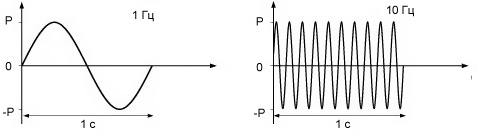
\includegraphics[width=0.7\linewidth]{images/frequency.png}
\caption{\label{fig:frequency}Гармонічний сигнал з частотою 1Гц(зліва) і 10Гц(справа).}
\end{figure}

\subsection{Потужність}
Визначення потужності як фізичної величини звучить наступним чином --- це робота, виконана за одиницю часу, або енергія, передана за одиницю часу. Вимірюється у Ватах (Вт). Також, коли ми будемо оперувати відносними величинами потужності, то часто зустрічатимемо потужність, позначену у dBm (децибел-міліват, див. наступну секцію \ref{sec:db}).


\subsection{Відносні величини}
\label{sec:db}
Коли потрібно порівнювати які-небудь величини, це можна зробити по-різному. Наприклад, можна розділити одне значення на інше і отримати порядок, який вказує, у скільки разів відрізняються значення. А якщо ми оперуємо абсолютними величинами, наприклад, \texttt{0.0000000001 - 100000000}, то відношення між двома такими величинами буде ще більшим, ніж фактичні значення.

Основна причина, чому використовуються децибели, полягає в тому, що фізична величина може змінюватися в дуже широкому діапазоні. Наприклад, співвідношення сигнал/шум (т.з. signal noise ratio або скорочено SNR) може бути настільки великим у абсолютному вираженні, що нам довелося б оперувати числами з багатьма нулями, що дуже незручно. Тому для таких величин і випадків використовують логарифмічну шкалу -- децибели. Важливо пам'ятати:
\begin{itemize}[noitemsep, topsep=8pt]
\item Децибели --- це відносне значення, яке показує порядок підсилення або затухання.
\item Шкала в децибелах нелінійна, тобто \texttt{10Дб} і \texttt{100Дб} фактична величина буде відрізнятися не в \texttt{10} разів, а в \texttt{1000 000 000}.
\item Негативне значення в \texttt{Дб} означає, що фактична величина не негативна, а лише менша за одиницю.
\end{itemize}


\subsection{dBm}
Також потрібно розуміти, що коли ми говоримо про децибели, то зазвичай це робимо у прив'язці до якоїсь фізичної величини. Наприклад, рівень потужності в децибелах відносно \texttt{1мВт} називається \textbf{dBm} (децибел-міліват).


\begin{table}[h!]
\centering
\begin{tabular}{|c|l||c|l|}
\hline
\textbf{dBm}  & \textbf{мВт} & \textbf{dBm} & \textbf{мВт} \\
\hline
100  & 10000000000  &  -1  & 0.794 \\
90   & 1000000000   &  -3  & 0.501  \\
80   & 100000000    &  -6  & 0.251  \\
70   & 10000000     & -10  & 0.1 \\
60   & 1000000      & -20  & 0.01 \\
50   & 100000       & -30  & 0.001 \\
40   & 10000        & -40  & 0.0001 \\
30   & 1000         & -50  & 0.00001 \\
20   & 100          & -60  & 0.000001 \\
10   & 10           & -70  & 0.0000001 \\
 6   & 3.981        & -80  & 0.00000001 \\
 3   & 1.995.       & -90  & 0.000000001 \\
 1   & 1.259        & -100 & 0.0000000001 \\
\hline
\end{tabular}
\caption{\label{table:dbm2mwatts}Співвідношення dBm до мВт}
\end{table}

Декілька прикладів:
\begin{itemize}[noitemsep, topsep=8pt]
\item Потужність WiFi роутера в середньому складає \texttt{17dBm} (приблизно \texttt{0.05Вт}).
\item Потужність мобільного телефона приблизно складає \texttt{33dBm} (приблизно \texttt{2Вт}).
\item Потужність антидронової рушниці складає \texttt{40dBm} (дорівнює \texttt{10Вт}).
\end{itemize}

На практиці співвідношення значень \texttt{dBm до мВт} зазвичай мало хто знає або пам'ятає на пам'ять --- це нормально. Для конвертації можна використовувати наведену Табл. \ref{table:dbm2mwatts} або онлайн калькулятори: \href{https://www.everythingrf.com/rf-calculators/dbm-to-watts}{dBm в Вт} та \href{https://www.everythingrf.com/rf-calculators/watt-to-dbm}{Вт в dBm}.
\subsection{dBi}


\textbf{dBi} (decibels isotropic) --- це одиниця вимірювання підсилення антен відносно \textit{еталонної} антени. За таку еталонну антена прийнято т.зв. ізотропний випромінювач — ідеальна антена, діаграма спрямованості якої є сферою, коефіцієнт підсилення дорівнює одиниці, а ККД — 100\%. Випромінювання сигналу такою антеною відбувається з рівномірною інтенсивністю в усі сторони. Такої антени в природі не існує, це віртуальний об'єкт, однак дуже зручний як еталон для вимірювання параметрів реальних антен.

Існує ще одна одиниця: dBd -- тут за еталон прийнято напівхвильовий диполь. Проте використання dBi є більш зручним, оскільки в цьому випадку легше проводити розрахунок енергетичного балансу. dBi -- це відносна одиниця, яка по суті нічим не відрізняється від звичайного децибела, за винятком визначення еталону, відносно якого ведеться відлік.

Принципової різниці між dBi і dBd немає -- підсилення в dBi = підсиленню в dBd + 2,15 dB. У старих радіоаматорських книжках і журналах підсилення антен вимірюють просто в децибелах. У такому випадку, найчастіше мається на увазі підсилення відносно напівхвильового вібратора, тобто воно еквівалентне dBd. Вимірювання відносно ізотропного випромінювача спочатку використовувалося тільки в США, але останнім часом поширилося по всьому світу, тому для уникнення плутанини зараз, якщо йдеться про підсилення антени, правилом гарного тону вважається використання децибела з суфіксом -- dBi або dBd.


\begin{itemize}[noitemsep, topsep=8pt]
\item \textbf{Ізотропний випромінювач} -- це ідеальна модель антени, яка випромінює однаково у всіх напрямках. Хоча такі антени не існують на практиці, їх використовують як базу для порівняння.
\item \textbf{Коефіцієнт підсилення} в dBi показує, наскільки антена спрямована. Наприклад, якщо антена має підсилення 6 dBi, це означає, що в певному напрямку вона випромінює в 4 рази більше енергії $(10^{\frac{6}{10}} \approx 4)$, ніж ізотропний випромінювач.
\item \textbf{Чим вищий показник} dBi, тим більш спрямованою є антена, що означає, що вона концентрує більше енергії в одному напрямку, але менше випромінює в інші.
\end{itemize}

\textbf{Приклад.} Антена з підсиленням 3 dBi випромінює приблизно вдвічі більше енергії в певному напрямку порівняно з ізотропним випромінювачем. Якщо підсилення антени становить 9 dBi, це означає, що антена має значно кращу спрямованість і концентрує енергію ще вужче в одному напрямку.

\section{Радіохвилі}

\textbf{Радіохвилі} -- це тип електромагнітного випромінювання з довжиною хвиль понад 1 мм (частотою нижче 300 ГГц). Неформально визначення радіохвиль можна пояснити як електромагнітну енергію у просторі. Це є основою для розуміння певних явищ радіохвиль, звісно, як аналогія.

\begin{figure}[h!]
\centering
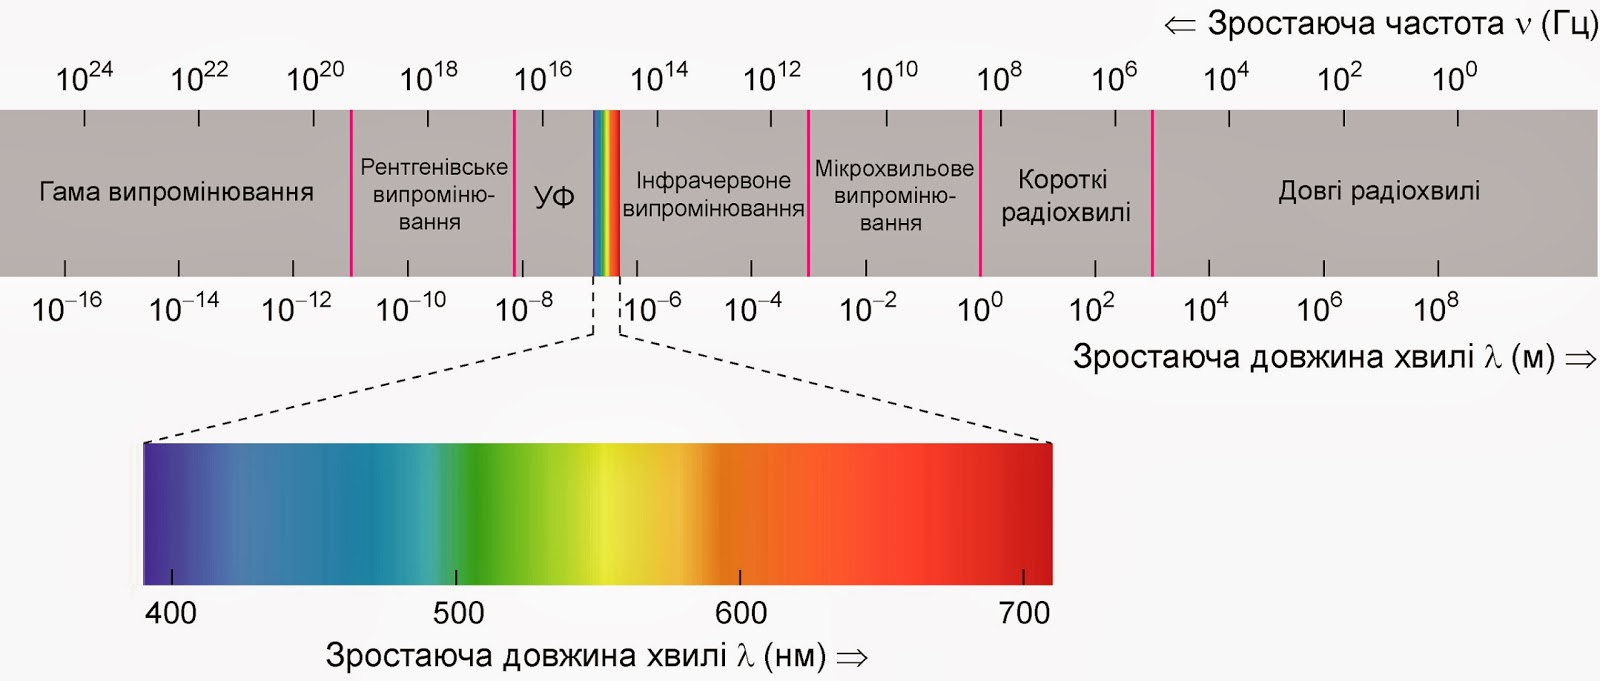
\includegraphics[width=0.9\linewidth]{images/electromagnetic-range.jpg}
\caption{\label{fig:electromagnetic}Діапазон радіохвиль на загальному спектрі електромагнітних хвиль.}
\end{figure}

Довжина хвилі може бути обчислена за адаптованою формулою:

\[
\lambda = \frac{300}{f}
\]

\begin{itemize}[noitemsep, topsep=8pt]
\item $\lambda$ -- довжина хвилі в метрах
\item ${f}$ -- частота хвилі в \texttt{МГц}
\end{itemize}

Коли ми говоримо про радіохвилі, то зазвичай оперуємо частотою в Гц з різними приставками (МГц, ГГц, тощо) -- але інколи можемо зустріти розмірність в метрах, міліметрах та сантиметрах. Якщо знаємо довжину хвилі і треба порахувати частоту, то виконуємо наступну послідовність -- переводимо довжину хвилі у метри, \texttt{300} ділимо на це значення (отримаємо частоту в МГц).

Розуміння довжини хвилі потрібно в контексті розміру антен. На практиці зустрічаються антени, розміри яких дорівнюють \texttt{$\lambda$/2} або \texttt{$\lambda$/4}.

\textbf{Приклад 1}. Для спектроаналізатора типу TinySA доволі часто використовується направлена логоперіодична антена на діапазон частот \texttt{600МГц - 6ГГц}. В цьому типі антен ширина кожного вібратора дорівнює \texttt{$\lambda$/2}. За формулою найширша частина антени буде \texttt{300/600МГц}, що дорівнює \texttt{0.5м} і відповідає повній довжині хвилі, а половина цього значення (\texttt{$\lambda$/2}) -- це \texttt{25см}.

\textbf{Приклад 2}. Ми знайшли ворожий дрон з антеною горизонтальної поляризації \href{https://modelistam.com.ua/images/dl-ant-rx60.jpg}{типу діполь}. Довжина антени складає \texttt{17.6см}. Питання: на яку частоту нам потрібен РЕБ? Спочатку переведемо сантиметри в метри, що дорівнює \texttt{0.176м}. Далі, знаючи, що для цього типу антен довжина складає половину довжини хвилі, то відповідна повна довжина буде \texttt{2*0.176 = 0.352м}. Щоб отримати робочу частоту керування дрона, застосовуємо формулу \texttt{300/0.352 = 852МГц}. Тобто, нам потрібен РЕБ на діапазон \texttt{800 - 900МГц}.

\subsection{Класифікація радіохвиль}

Торкаючись теми радіохвиль, варто розібратись із термінологію, яку використовують для їх класифікації. Класифікація радіохвиль відбувається за діапазонами частот.

\begin{table}[ht]
	\centering
	\begin{tabular}{|l|l|l|}
		\hline 
		\textbf{Найменування}  & \textbf{Повна назва} & \textbf{Діапазони} \\
		\hline
		VLF      	& Very low frequencies		& 3 - 30 kHz   		\\
		LF    		& Low frequencies    		& 30 - 300 kHz 		\\
		MF			& Medium frequencies		& 300 - 3000 kHz	\\
		HF    		& High frequencies			& 3 - 30 MHz 		\\
		VHF     	& Very high frequencies 	& 30 - 300 MHz  	\\
		UHF			& Ultra high frequencies	& 300 - 3000 MHz	\\
		SHF			& Super high frequencies	& 3000 - 30000 MHz 	\\
		\hline
	\end{tabular}
	\caption{\label{table:radiowaves_types} Таблиця класифікації радіохвилі по діапазонам}
\end{table}

Із цієї номенклатури класифікацій нас більше усього цікавлять хвилі в діапазонах VHF, UHF та частково SHF до 6-8 GHz.  Найменування потрібно знати, бо у більшості випадків робота пристроїв визначається саме по такому принципу, як приклад, можна розглянути радіостанції, які працюють в діапазонах VHF або UHF, або в обох діапазонах. Отримавши цю інформацію, ви будете знати про які діапазони конкретно йде мова, або в яких діапазонах треба проводити якусь роботу.


\subsection{Розповсюдження радіохвиль}

Природа розповсюдження радіохвиль у просторі дуже залежить від фізичних властивостей хвилі, а саме від її частоти та довжини. Хвилі різної довжини мають різну природу поширення у просторі, а саме проникаючі властивості та властивості оминати перешкоди. Враховуючи ці обосливості під різні частотні діапазони використовуються різні шляхи передачі інформації.

\begin{figure}[h!]
	\centering
	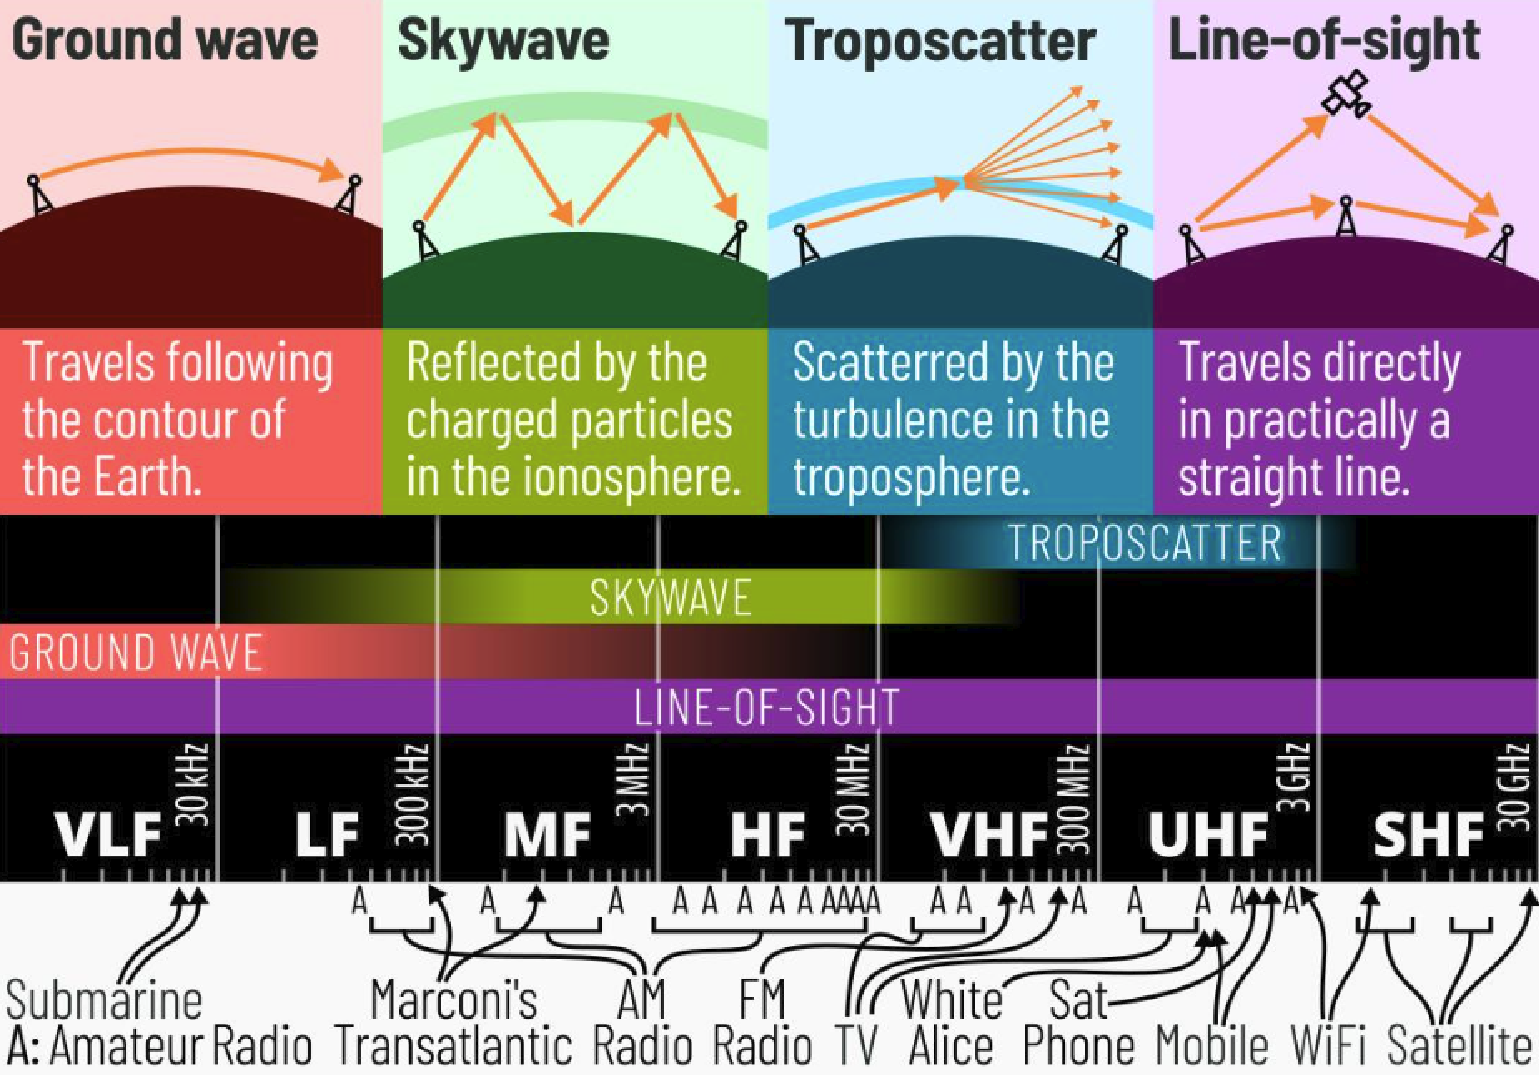
\includegraphics[width=0.8\linewidth]{images/radio-propagation.png}
	\caption{\label{fig:radio-propagation} Розповсюдження радіохвиль}
\end{figure}


\begin{itemize}[noitemsep, topsep=8pt]
	\item Для діапазонів VLF, LF, MF передача інформації може відбувається вздовж контура землі або навіть під водою. Довжина хвиль в цих діапазонах може сягати кілометрів, а то і десятків для VLF діапазону. Враховуючи ці властивості, вони мають особливість дуже далеко розповсюджуватись та оминати гарно перешкоди забезпечуючи зв'язок на дуже далеких відстанях. 
	\item Радіохвилі в діапазонах частоково LF, MF, HF та частоков VHF мають вже коротші довжини хвиль і механіка передачі інформації відбувається вже за іншими принципами, а саме за рахунок відбиття їх від іоносфери.
	\item Радіохвилі в діапазонах VHF та UHF вже мають різні характеристики поширення у просторі. VHF хвилі поширюються по прямолінійній траєкторії, і тому передача інформації дуже залежить від зони прямої видимості між передавачем і приймачем. UHF хвилі також поширюються по прямолінійній траєкторії, але вони мають особливість краще відбиваються від природних і штучних об'єктів. Хвилі в цих діапазонах також поширюються на значні відстані за рахунок рефракції та розсіювання у тропосфері.
	\item Передача інформації для SHF відбуваєтся лише в межах прямої відимості між передавачем та приймачем.
\end{itemize}

Як ми вже зрозуміли, що природа поширення радіохвиль для різних частот буде різна, але для всих цих діапазонів працює одне основне правило, що їх поєднує, а саме те, що незалежно від діапазону передача інформація може відбуватись в зоні прямої видимості. Тому ми наближаємось до поняття радіогоризонту.   

\textbf{Радіогоризонт} -- це максимальна відстань від антени до точки на земній поверхні, де радіохвилі ще можуть бути прийняті при прямій видимості. Іншими словами, це межа, за яку радіосигнал перестає поширюватися по прямій лінії через кривизну Землі. Радіогоризонт збільшується з висотою антени або розташування її на максимальній висоті. Чим вище антена, тим далі поширюється сигнал.

\begin{figure}[h!]
\centering
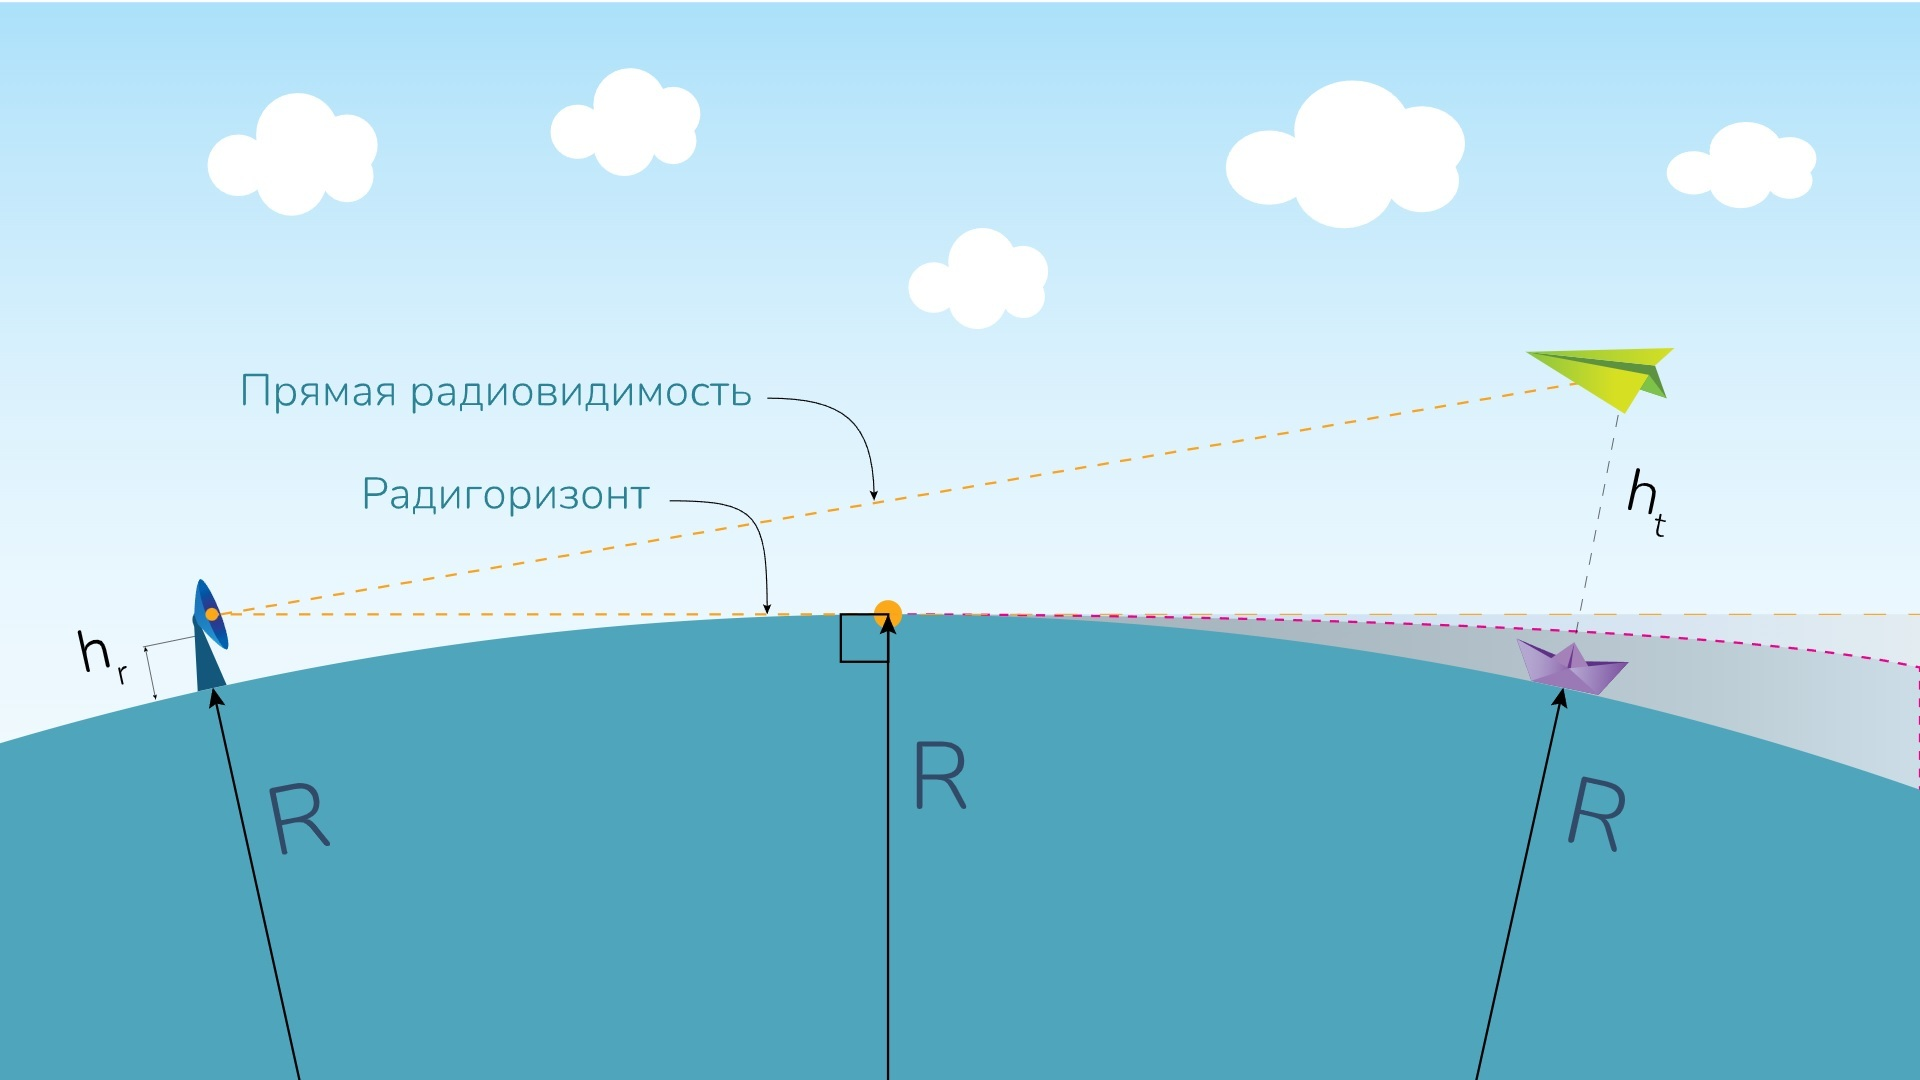
\includegraphics[width=0.6\linewidth]{images/radio-horizon.jpeg}
\caption{\label{fig:radio-horizon}Радіогоризонт}
\end{figure}

\subsection{Рефлексія радіохвиль}

\textbf{Рефлексія радіохвиль} --- це відбиття радіохвиль від перешкод, яке призводить до зміни напрямку розповсюдження радіохвилі. В залежності від задачі це може мати, як і позитивні, так і негативні наслідки. Але в контексті радіоелектророзвідки, а саме пеленгаційних систем, це ускладнює процес визначення оригінального напрямку джерела раідовипромінювача, осболиво, якщо вібиття відбувається хаотично в різні напрямки, що приводить до ситуації, коли одне і те самє радіоджерело надходить з різних напрямків. Такє відбиття називається дифузним, але відбиття також може бути і дзеркальним. 

\begin{figure}[h!]
	\centering
	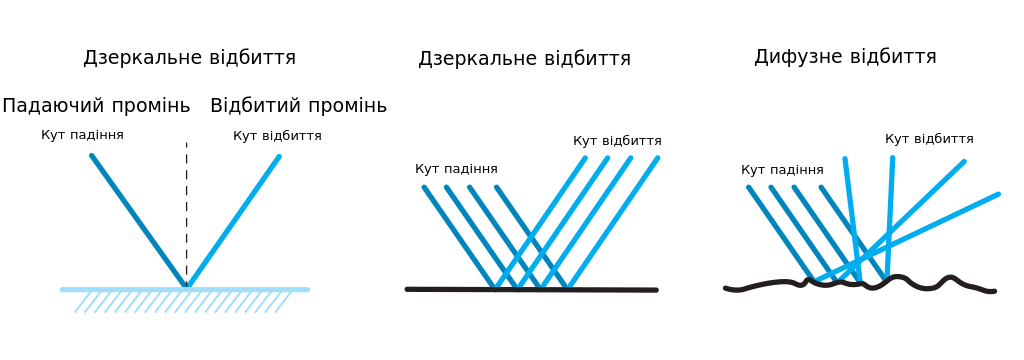
\includegraphics[width=0.8\linewidth]{images/reflection.png}
	\caption{\label{fig:reflection}Рефлексія радіохвиль}
\end{figure}

Дзеркальне відбиття має доволі просту природу і визначається тим, що кут падіння проміню буде відповідати куту його відиття, тобто кути будуть дзеркально-симетричними. Наприклад, якщо ви працюєте за пеленгатором і знаєте, що джерело радіовипромінювання знаходиться за певним напрямком, але пеленгаційна система визначає його, як протилежний у 180 градусів від очікуваного, то ви точно зіткнулись із перевідбиттям. Радіохвилі можуть відбиватися від різних поверхонь, таких як земля, будівлі, металеві предмети, водойоми та предмети, що утримують в собі вологу.

\newpage
\subsection{Рефракція радіохвиль}

\textbf{Рефракція радіохвиль} --- це зміна траєкторії радіохвилі під впливом середовища. Температура, тиск і вологість впливають на швидкість поширення радіохвиль у просторі, як результат на зміну напрямку для VHF та UHF діапазонів. Швидкість поширення хвиль в різних середовищах різна, як б це дивно не звучало, довжина хвилі в цьому випадку теж міняється, але тут варто зазначити, що це ніяким чином не впливає на її частоту.  

\begin{figure}[h!]
	\centering
	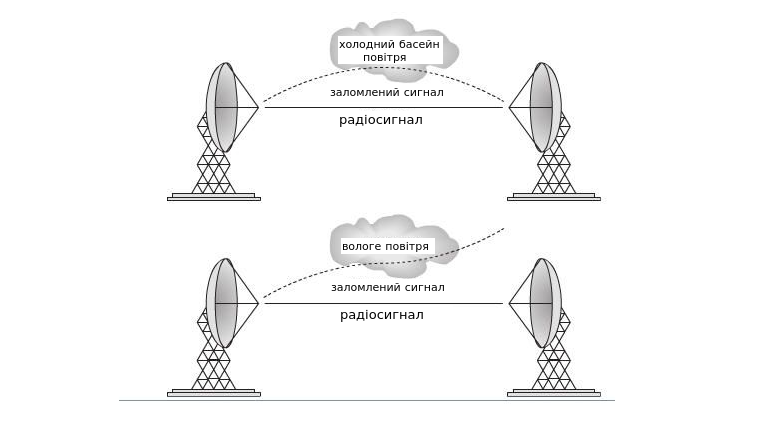
\includegraphics[width=0.8\linewidth]{images/refraction.png}
	\caption{\label{fig:refraction}Рефракція радіохвиль}
\end{figure}


Завдяки такій фізичній властивості, ми можемо відправляти інформацію на дуже далекі відстані за раідогоризонт, оминати перешкоди за рахунок заломлення радіохвиль від іоносфери для HF діапазону.

\begin{figure}[h!]
	\centering
	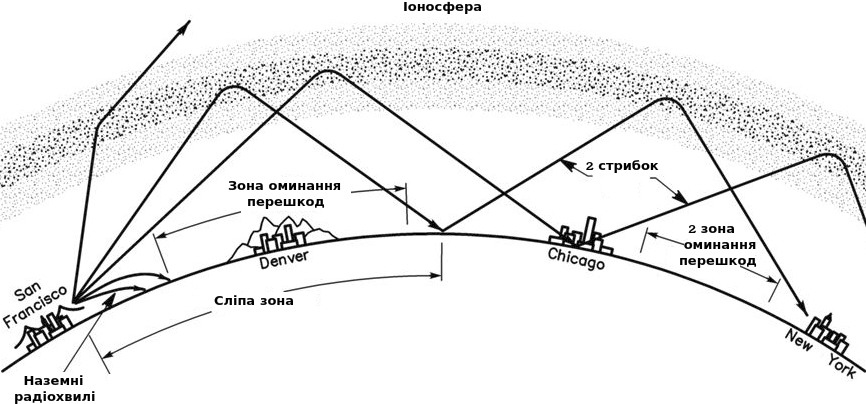
\includegraphics[width=0.8\linewidth]{images/refraction2.png}
	\caption{\label{fig:refraction2}Рефракція в іоносфері}
\end{figure}



\subsection{Дифракція радіохвиль}

\textbf{Дифракція радіохвиль} --- це здатність радіохвиль оминати перешкоди на своєму шляху, що дозволяє досягати сліпих зон, але при цьому істотно втрачати потужність. Тут варто зазначити, що дифракці має пряму залежність від довжини хвилі, чим більше довжина хвилі і меньше частота, тим краще вона долає перешкоди, тобто хвилі в діапазонах HF, VHF краще огинають перешкоди ніж в діапазонах UHF. Сам ефект, зазвичай, може проявлятись в момент при зіткненні хвилі об края перешкод або при проходженні хвилі через щілини. Радіохвилі також здатні буквально огинати перешкоди на своєму шляху, але за умови, якщо перешкода є меньшою за довжину хвилі.

\begin{figure}[h!]
	\centering
	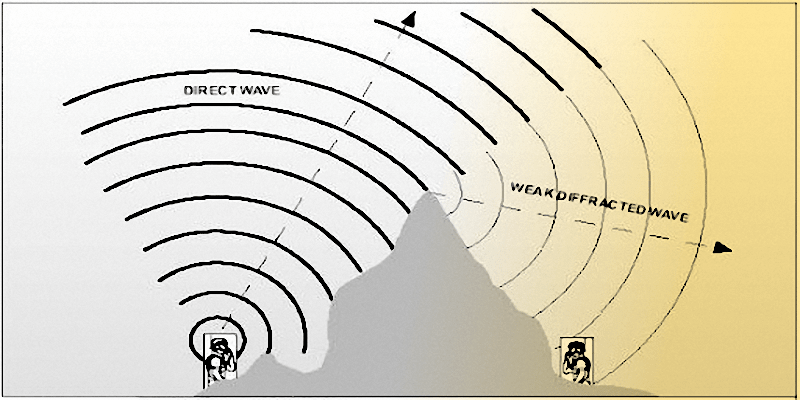
\includegraphics[width=0.8\linewidth]{images/diffraction.png}
	\caption{\label{fig:diffraction}Дифракція та перешкоди}
\end{figure}

Окрім позитивних ефектів, він також має і негативний для пеленгаційних систем, бо є хибним азимутом джерела випромінювання. Огинаючи перешкоди радіохвиля міняє свій істиний азумут і як у випадку з рефракцією та рефлексією створює хибний кут джерела випромінювання. 
\begin{figure}[h!]
	\centering
	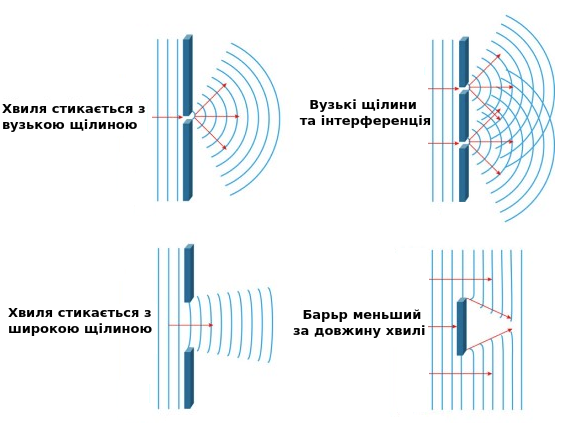
\includegraphics[width=0.6\linewidth]{images/diffraction_all.png}
	\caption{\label{fig:diffraction_all} Дифракція радіохвиль}
\end{figure}

\subsection{Інтерференція радіохвиль}

\textbf{Інтерференція радіохвиль} --- це явище, яке взаємно збільшується або зменшується в результаті підсумовування амплітуд хвиль, що поширюються в просторі. Результат інтерференції залежить від різниці фаз: в одному випадку амплітуда збільшується (співпадіння по фазі, мал. \ref{fig:interferense} зліва), а в іншому зменшується (хвилі в протифазі, мал. \ref{fig:interferense} справа).

\begin{figure}[h!]
\centering
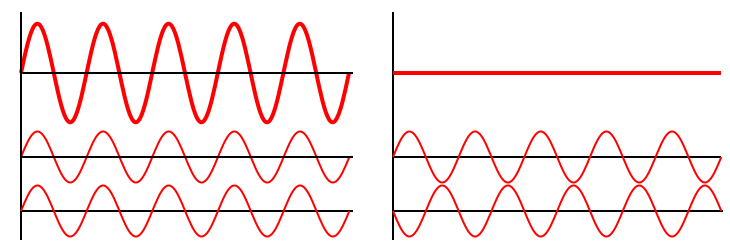
\includegraphics[width=0.7\linewidth]{images/interferense.png}
\caption{\label{fig:interferense}Інтерференція радіохвиль}
\end{figure}

Наприклад, в контексті РЕБ-у,якщо антени модуля РЕБ будуть близько розташовані і які будуть працювати на одному або суміжних діапазоні, можуть значно зменшувати ефективність подавлення через вплив одна на одну, коли радіохвилі випромінюються у протифазі. Як наочний приклад такої взаємодії хвиль можна спостерігати у природі, наприклад, на поверхні води, коли хвилі від різних джерел впливають одна на одну (мал. \ref{fig:two-emmitions}).

\begin{figure}[h!]
\centering
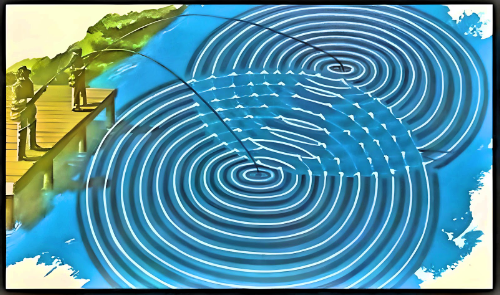
\includegraphics[width=0.6\linewidth]{images/two-emmitions.png}
\caption{\label{fig:two-emmitions}Взаємний вплив різних джерел хвиль.}
\end{figure}

\subsection{Федінг радіохвиль}

\textbf{Федінг радіохвиль} --- це саме звичайне затухання радіохвиль у просторі. Тут більше мова йде не про природне згасання по потужності відностно відстані, а про більш складний комплексний процес. Тут більше мова про сумарний ефект усих явищ, які ми розглядали перед цим. Справа у тому, що сигнал надходить до приймача кількома шляхами, а саме із-за перевідбитів, дифракцій та розсіювань ці шляхи мають різну довжину, тому сигнали надходять в різних фазах. Коли ці сигнали попадають у фазу, то сигнал посилюється. Коли вони деструктивно інтерферують, тобто попадають у протифазу, вони компенсують один одного, спричиняючи згасання, що і є федінгом. \textbf{Приклад}: Уявіть, що ви йдете містом зі своїм телефоном. Ви знаходитесь у місці, де на ваш телефон потрапляє як прямий, так і відбитий сигнал. Коли ви рухаєтесь на кілька сантиметрів, сигнали можуть переходити від конструктивних до деструктивних перешкод і приходити у протифазі на ваш телефон. Рівень сигналу, що відображається на вашому телефоні, коливається — це і той самий федінг. Тут ми підходимо до поняття інтерференції радіохвиль.

\subsection{Зона Френеля}

\textbf{Зона Френеля} --- це еліптична область, що оточує лінію прямої видимості, яка з'єднує дві точки бездротової мережі. Між цими двома точками електромагнітна хвиля набуває форми еліпсоїда, він формується навколо лінії видимості (Line-of-Sight). Для гарної якості сигналу різні перешкоди місцевості (елементи рельєфу, будівлі, дерева) не повинні перетинати не тільки лінію прямої видимості, а і зону Френеля.  Максимальний радіус еліпсоїда у центральній частині, залежить від двох параметрів - частоти та відстані. Знаючи частоту та відстань між точками, можна розрахувати максимальний радіус зони Френеля у центральній точці між двома антенами.

\begin{figure}[h!]
	\centering
	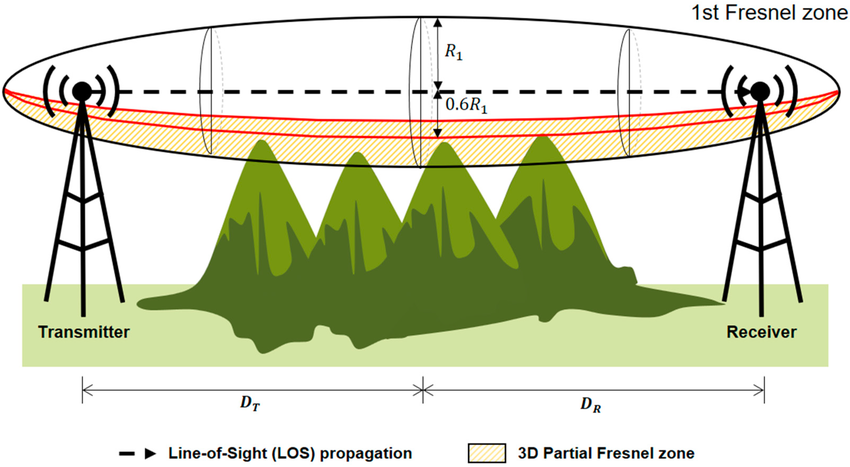
\includegraphics[width=0.9\linewidth]{images/fresnel-zone.png}
	\caption{\label{fig:fresnel-zone} Зона Френеля.}
\end{figure}

Зону Френеля потрібно знати і вміти розраховувати, бо це дає розуміння, як будувати зв'язок за рахунок WIFI мостів, або інших меш мереж, комунікацій між наземною станцію та БПЛА, а також для ефективного застосування РЕБ-у. Для себе можно визначаити оптимальне правило, що 60 відсотків першої зони Френеля повинно бути вільним від перешкод, якщо ми хочемо мати більш-менш стабільну передачу інформації. Розрахувати зону Френеля в метрах можно за наступною формулою:


\[
R_1 = 17.32 \cdot \sqrt{\frac{d_t \cdot d_r}{f \cdot (d_t + d_r)}}
\]

\begin{itemize}[noitemsep, topsep=8pt]
	\item $R1$ -- перша зона Френеля
	\item $dt,dr$ -- відстані до точки центру зони від передавача та приймача (у \texttt{км})
	\item ${f}$ -- частота в \texttt{GHz}
\end{itemize}

\textbf{Приклад}: Відстань між точками складає 1 км, частота - 2.4 Ghz і робимо наступні розрахунки за формулою.

\[
R_1 = 17.32 \cdot \sqrt{\frac{0.5 \cdot 0.5}{2.4 \cdot (0.5 + 0.5)}}=17.32 \cdot \sqrt {\frac{0.25}{2.4}}=5.59 м
\]

Відстань між двома антенами складає 1 км, відповідно відстань до центру буде складати по 0.5 км. Застосувавши формулу, ми визначили радіус першої зони Френеля і він складає 5.59 метри. Попередньо було зазначено, що мінімальна необхідна зона без перешкод має складати мінімум 60 відсотків від першої зони, при якій буде присутня передача інформації. Відповідно, мінімальний радіус без перешкод в центральній частині від зони прямої видимості має складати 3.35 метри.


\section{Модуляція}
\label{sec:modulation}

\textbf{Модуляція} --- це процес зміни одного або кількох параметрів високочастотного сигналу (який називається носієм) під впливом іншого сигналу, що несе інформацію (наприклад, керування дроном або відеосигнал). Модуляція використовується для передачі інформації на великі відстані через різні канали зв'язку. У контексті нашої теми, коли ми говоримо про модуляцію, то маємо на увазі радіохвилі, але важливо зауважити, що це загальне поняття і модуляція може здійснюватися на інших фізичних принципах, наприклад, за допомогою світла в оптичному кабелі. Радіохвиля володіє трьома головними характеристиками, якими її можно описати, а саме амплітудою, фазою та частотою і за рахунок зміни цих характеристик по окремості, або навіть в комбінації між собою, за певними алгоритмами дозволяє нам передавати інформацію. Торкаючись теми модуляції, ми повинні розуміти, що існує і зворотній процес, який називається демодуляцією. 

\begin{figure}[h!]
	\centering
	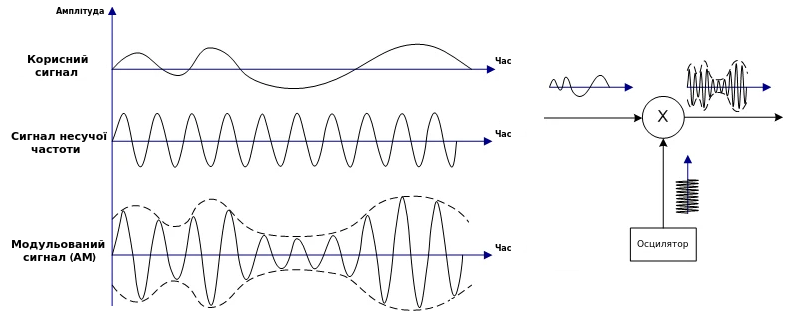
\includegraphics[width=0.9\linewidth]{images/modulation_signal.png}
	\caption{\label{fig:modulation_signal} Модуляція сигналу}
\end{figure}

\textbf{Демодуляція} --- це процес вилучення оригінального інформаційного корисного сигналу з модульованої несучої хвилі. Демодуляція є основною функцією всіх радіоприймачів, телевізорів та комунікаційних приймачів. 
Вцілому модуляція ділиться на два типи: аналогова та цифрова і тут варто пояснити принципову різницю між ними.

В рамках цього блоку ми розглянемо лише базові типи аналоговихта цифривоих модуляцій \footnote{Детальніше питання базових типів модуляцій розкрито у відео, яке можна \href{https://www.youtube.com/watch?v=gfz1FbIOMbs}{переглянути за посиланням}.}. Більш складні типи модуляції --- це по суті комбінація базових типів, розуміючи їх, відносно легко розібратися з іншими.


\subsection{Аналогова модуляція}
\textbf{Аналогова модуляція} --- це процес передачі аналогового низькочастотного базового сигналу через високочастотний несучий аналоговий сигнал. В аналоговій модуляції, як несучий, так і інформаційний, він же корисний сигнал, є аналоговими хвилями. Передача інформації в аналоговій модуляції виконується за рахунок зміни характеристики одного із параметрів, а саме амплітуди, фази або частоти, але також існують і комбінації зі змін цих характеристик.

\subsubsection{Амплітудна модуляція}
\textbf{Амплітудна модуляція} (АМ) --- це метод модуляції, що використовується для передачі інформації шляхом зміни амплітуди сигналу-носія відповідно до миттєвого значення сигналу повідомлення (мал. \ref{fig:am}).

\begin{figure}[h!]
\centering
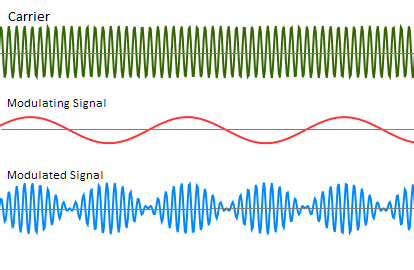
\includegraphics[width=0.6\linewidth]{images/am.png}
\caption{\label{fig:am}Амплітудна модуляція.}
\end{figure}

\begin{itemize}[noitemsep, topsep=8pt]
\item \textbf{Сигнал-носій}: Це високочастотний сигнал постійної амплітуди, частота якого не змінюється під час передачі інформації. Позначений зеленим.
\item \textbf{Модулюючий сигнал}: Це інформаційний сигнал, який несе корисну інформацію (наприклад, керування дроном). Він має відносно низьку частоту порівняно з сигналом-носієм. Позначений червоним.
\item \textbf{Процес модуляції}: Амплітуда сигналу-носія змінюється залежно від амплітуди модулюючого сигналу. Чим вища амплітуда модулюючого сигналу, тим більше змінюється амплітуда носія.
\end{itemize}

\subsubsection{Частотна модуляція}

\textbf{Частотна модуляція} (FM) --- це метод модуляції, при якому частота сигналу-носія змінюється відповідно до амплітуди модулюючого сигналу (інформаційного сигналу). Іншими словами, в процесі частотної модуляції амплітуда сигналу-носія залишається незмінною, а частота коливається залежно від миттєвого значення інформаційного сигналу (мал. \ref{fig:fm}).

\begin{figure}[h!]
\centering
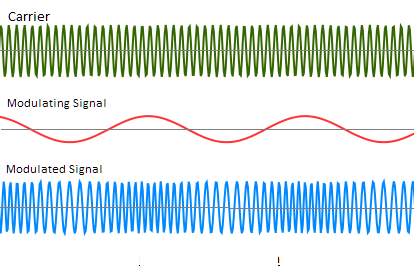
\includegraphics[width=0.6\linewidth]{images/fm.png}
\caption{\label{fig:fm}Частотна модуляція.}
\end{figure}

\begin{itemize}[noitemsep, topsep=8pt]
\item \textbf{Сигнал-носій}: Це високочастотний сигнал, частота якого змінюється в процесі модуляції, але амплітуда залишається постійною. Позн. зеленим.
\item \textbf{Модулюючий сигнал}: Це сигнал, який несе інформацію (наприклад, аудіо). Його амплітуда визначає, на скільки зміниться частота сигналу-носія. Позн. червоним.
\item \textbf{Процес модуляції}: Частота сигналу-носія збільшується, коли амплітуда модулюючого сигналу зростає, і зменшується, коли амплітуда падає. Це відхилення частоти називається \textit{девіацією частоти}.
\end{itemize}

\subsubsection{Фазова модуляція}

\textbf{Фазова модуляція} (PM) --- це метод модуляції, при якому фаза сигналу-носія змінюється відповідно до амплітуди модулюючого сигналу (інформаційного сигналу). На відміну від амплітудної або частотної модуляції, в фазовій модуляції основним параметром, що змінюється, є фаза сигналу(мал. \ref{fig:pm}).

\begin{figure}[h!]
\centering
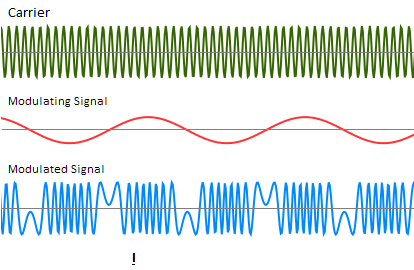
\includegraphics[width=0.6\linewidth]{images/pm.png}
\caption{\label{fig:pm}Фазова модуляція.}
\end{figure}

\begin{itemize}[noitemsep, topsep=8pt]
\item \textbf{Сигнал-носій}: Це високочастотний сигнал, фаза якого змінюється в процесі модуляції, тоді як частота і амплітуда залишаються постійними. Позначений зеленим.
\item \textbf{Модулюючий сигнал}: Це інформаційний сигнал, амплітуда якого визначає, наскільки змінюється фаза сигналу-носія. Позначений червоним.
\item \textbf{Процес модуляції}: Коли амплітуда модулюючого сигналу змінюється, фаза сигналу-носія також змінюється пропорційно до цієї амплітуди. Зміна фази може бути прямою або від'ємною залежно від того, як змінюється модулюючий сигнал.
\end{itemize}

\subsection{Цифрова модуляція}
\textbf{Цифрова модуляція} --- це процес передачі цифрового низькочастотного базового сигналу через високочастотний несучий аналоговий сигнал. Цифрова модуляція дещо схожа на аналогову модуляцію, за винятком того, що сигнал базової смуги має дискретний рівень амплітуди. Для двійкового сигналу він має лише два рівні: високий тобто логічна 1, або низький - логічний 0. Відповідно для цифрового сигналу ми робимо трансформацію корисної інформації в двійкові значення 1 та 0 і потім вже робимо модулювання цифрового сигналу на несучий аналоговий сигнал. Тут також варто пояснити, що є модуляція і маніпуляція. Фактично, обидва терміни стосуються одного й того ж процесу, але з деякими відмінностями. Концепція модуляції використовується для аналогових сигналів, а маніпуляції – для дискретних сигналів.

\subsubsection{Амплітудна маніпуляція}
\textbf{Амплітудна маніпуляція}(ASK) --- це техніка, за якої амплітуда несучої хвилі змінюється відповідно до переданих цифрових даних. Частота та фаза залишаються постійними, змінюється лише амплітуда. 

\begin{figure}[h!]
	\centering
	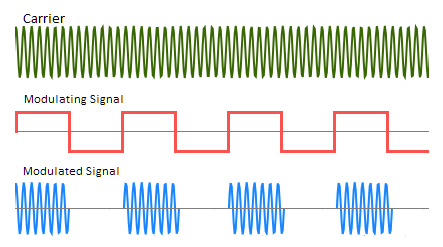
\includegraphics[width=0.6\linewidth]{images/ask.png}
	\caption{\label{fig:ask}Амплітунда маніпуляція.}
\end{figure}

\subsubsection{Частотна маніпуляція}
\textbf{Частотна маніпуляція}(FSK) --- це метод цифрової модуляції, при якому частота несучого сигналу змінюється відповідно до переданих бітів. Амплітуда і фаза залишаються сталими. Це більш надійний метод у шумових середовищах порівняно з амплітудною маніпуляцією.

\begin{figure}[h!]
	\centering
	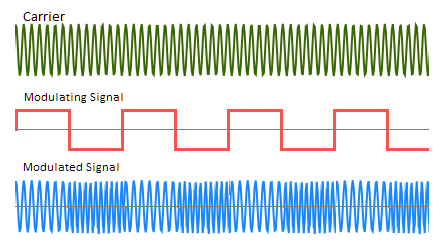
\includegraphics[width=0.6\linewidth]{images/fsk.png}
	\caption{\label{fig:fsk}Частотна маніпуляція.}
\end{figure}

\subsubsection{Фазова маніпуляція}
\textbf{Фазова маніпуляція}(PSK) --- це метод цифрової модуляції, при якому фаза несучого сигналу змінюється залежно від переданих бітів. Амплітуда та частота при цьому залишаються сталими. Цей тип маніпуляції потребує точної синхронізації фаз між передавачем та приймачем, але він є і більш ефективний з точки зору пропускної здатності, ніж ASK або FSK.

\begin{figure}[h!]
	\centering
	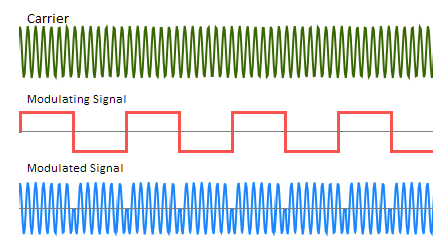
\includegraphics[width=0.6\linewidth]{images/psk.png}
	\caption{\label{fig:psk}Фазова маніпуляція.}
\end{figure}

Три основні методи цифрової модуляції: ASK, FSK та PSK можуть бути використані для передачі одного біта даних (0 або 1) за одиницю часу передачі. Цей метод називається двійковою маніпуляцією зі зсувом (B-ASK, B-FSK або B-PSK). Але оскільки несуча частота є обмеженим ресурсом, метод модуляції кількох бітів в одному часовому інтервалі часто є більш вигідним. У цьому методі кілька бітів даних групуються разом і кодуються в символи. Кожен символ призначається певному рівню модуляції. Ми називаємо ці схеми багаторівневою модуляцією. Якщо згрупувати біти по два, то кожен символ містить по 2 біти. Якщо до символу вдається маніпуляція, результуюча швидкість передачі даних подвоюється, і тоді ми маємо чотири різні символи: 00, 01, 10 та 11 (наприклад 4-PSK або 4-ASK). Якщо згрупувати бітовий потік по чотири, то ми маємо 16 різних символів: 0000, 0001, 0010… до 1111 (наприклад 16-QAM). Все це визначає швидкість передачі даних, яку також називають бітовою швидкістю (бітів за секунду або біт/с). Ми можемо спробувати ще більше збільшити бітову швидкість, але чим складніші символи, тим важче їх розрізняти на стороні приймача.

\begin{figure}[h!]
	\centering
	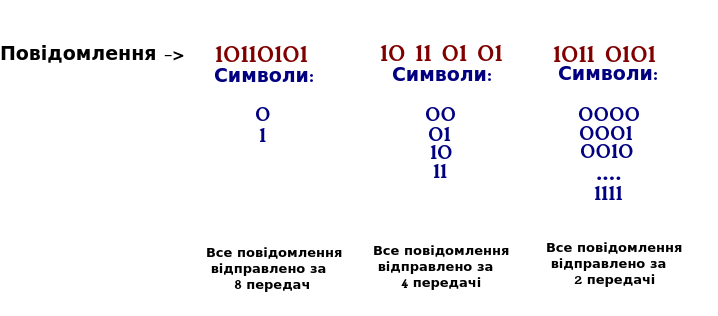
\includegraphics[width=0.8\linewidth]{images/transmittion_speed.png}
	\caption{\label{fig:transmittion_speed} Передача даних в залежності від бітрейту.}
\end{figure}

\begin{figure}[h!]
	\centering
	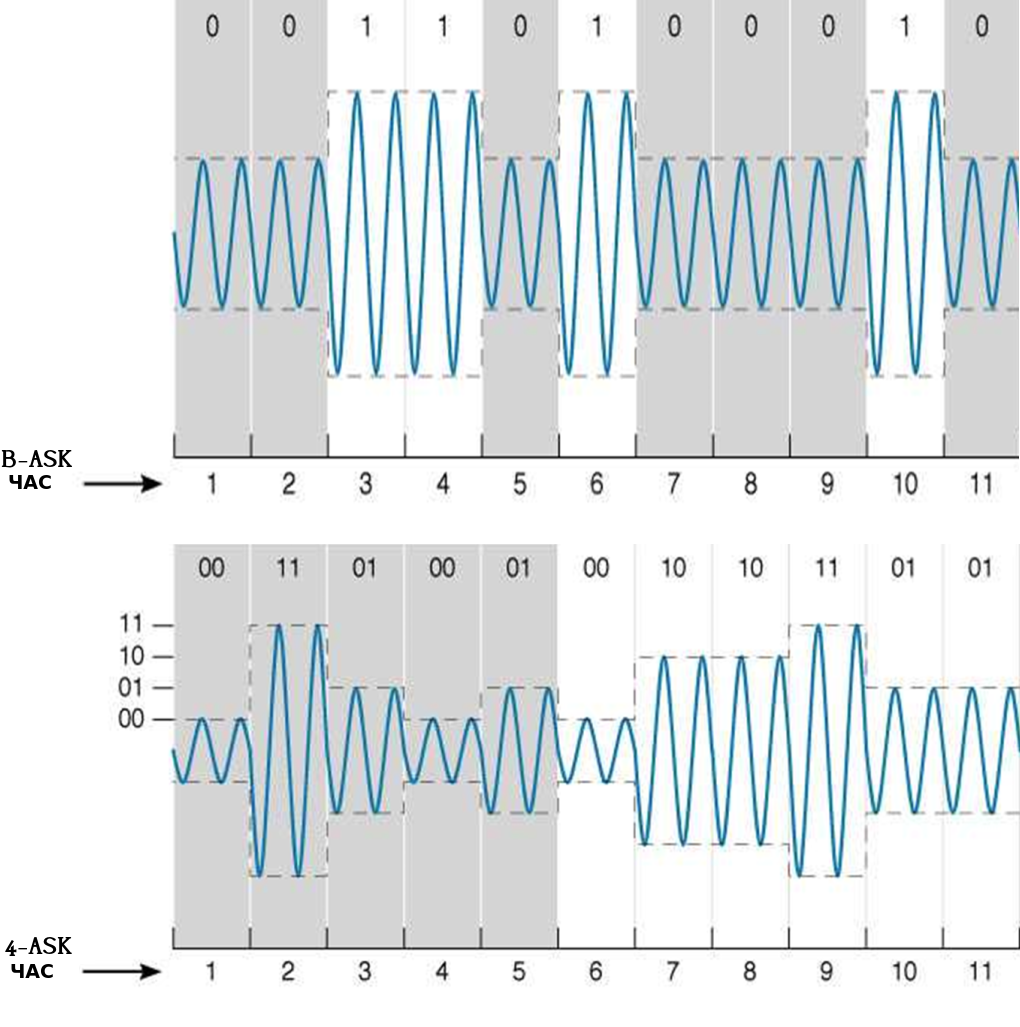
\includegraphics[width=0.8\linewidth]{images/comparison-bask-vs-4ask.png}
	\caption{\label{fig:comparison-bask-vs-4ask} Порівняння передачі данних для B-ASK та 4-ASK.}
\end{figure}


\newpage
\subsubsection{Квадратнурна амплітудна маніпуляція}
\textbf{Квадратнурна амплітудна маніпуляція}(QAM) --- це метод маніпуляції, який поєднує дві несучі хвилі, кожна з різною амплітудою та фазою, але з однією частотою для ефективної передачі даних. Визначення QAM полягає в кодуванні цифрових даних в аналогові сигнали, що дозволяє ефективно передавати інформацію по каналах зв'язку. Цей метод модуляції, який одночасно змінює амплітуду двох несучих хвиль, що знаходяться протифазі на 90 градусів. Таке поєднання амплітудної та фазової модуляції робить QAM особливо потужною, оскільки вона може представляти кілька бітів інформації на символ, збільшуючи пропускну здатність даних. Цей тип модулії також відносно необмежений по бітрейту, тому інсуюють різні різновиди QAM, наприклад: QAM-4 (2 біта), QAM-8(3 біта), QAM-16(4 біта), QAM-64 (6 бітів) і т.д.

\begin{figure}[h!]
	\centering
	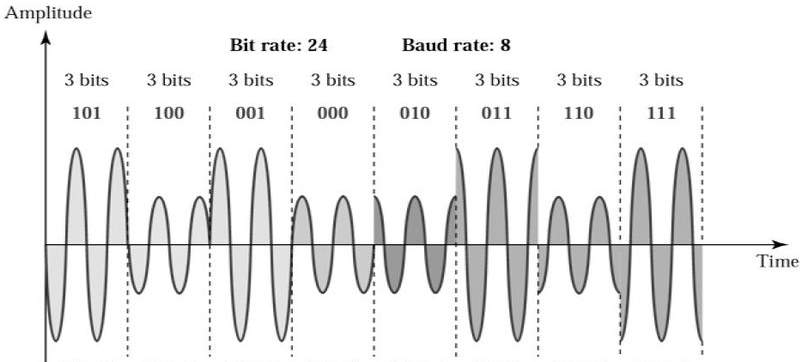
\includegraphics[width=0.8\linewidth]{images/qam.png}
	\caption{\label{fig:qam} QAM-8 модуляція.}
\end{figure}


\subsection{Ортогональне частотне мультиплексування}
\textbf{Ортогональне частотне мультиплексування} (OFDM): OFDM – це метод цифрової модуляції, який розділяє доступну смугу частот на кілька ортогональних піднесучих, кожна з яких модульована з низькою швидкістю передачі даних, що дозволяє ефективно передавати сигнали з високою швидкістю передачі даних у багатопроменевому середовищі.
Ортогональні сигнали – це сигнали, перпендикулярні один до одного. Основною властивістю ортогональних сигналів є те, що вони не перешкоджають один одному. Для роботи OFDM потрібна дуже точна синхронізація між вузлами, що здійснюють зв'язок. Якщо в підпотоках виникає відхилення частоти, вони більше не будуть ортогональними, через що виникатимуть інтерференції між сигналами. Це можно уявити собі як паралельну передачу багатьох низькошвидкісних сигналів на різних частотах — разом вони утворюють високошвидкісний канал передачі даних.

\begin{figure}[h!]
	\centering
	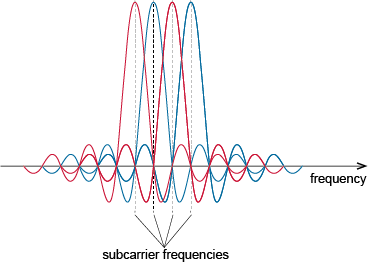
\includegraphics[width=0.7\linewidth]{images/ofdm.png}
	\caption{\label{fig:ofdm}  Приклад OFDM.}
\end{figure}


\subsection{ППРЧ}

\textbf{ППРЧ} (Перестроювання по частоті із псевдовипадковою перебудовою частоти) -- це метод радіозв'язку, при якому частота передавача змінюється за певним законом, зазвичай у псевдовипадковій послідовності. Така техніка використовується для підвищення стійкості зв'язку до перешкод, запобігання перехопленню, а також для кращого використання спектра.

Основна ідея ППРЧ полягає в тому, що передавач і приймач узгоджено \textit{перестрибують} між частотами в заздалегідь визначеному порядку. Якщо сторонній слухач не знає цієї послідовності, він не зможе прийняти корисний сигнал.

\begin{figure}[H]
\centering
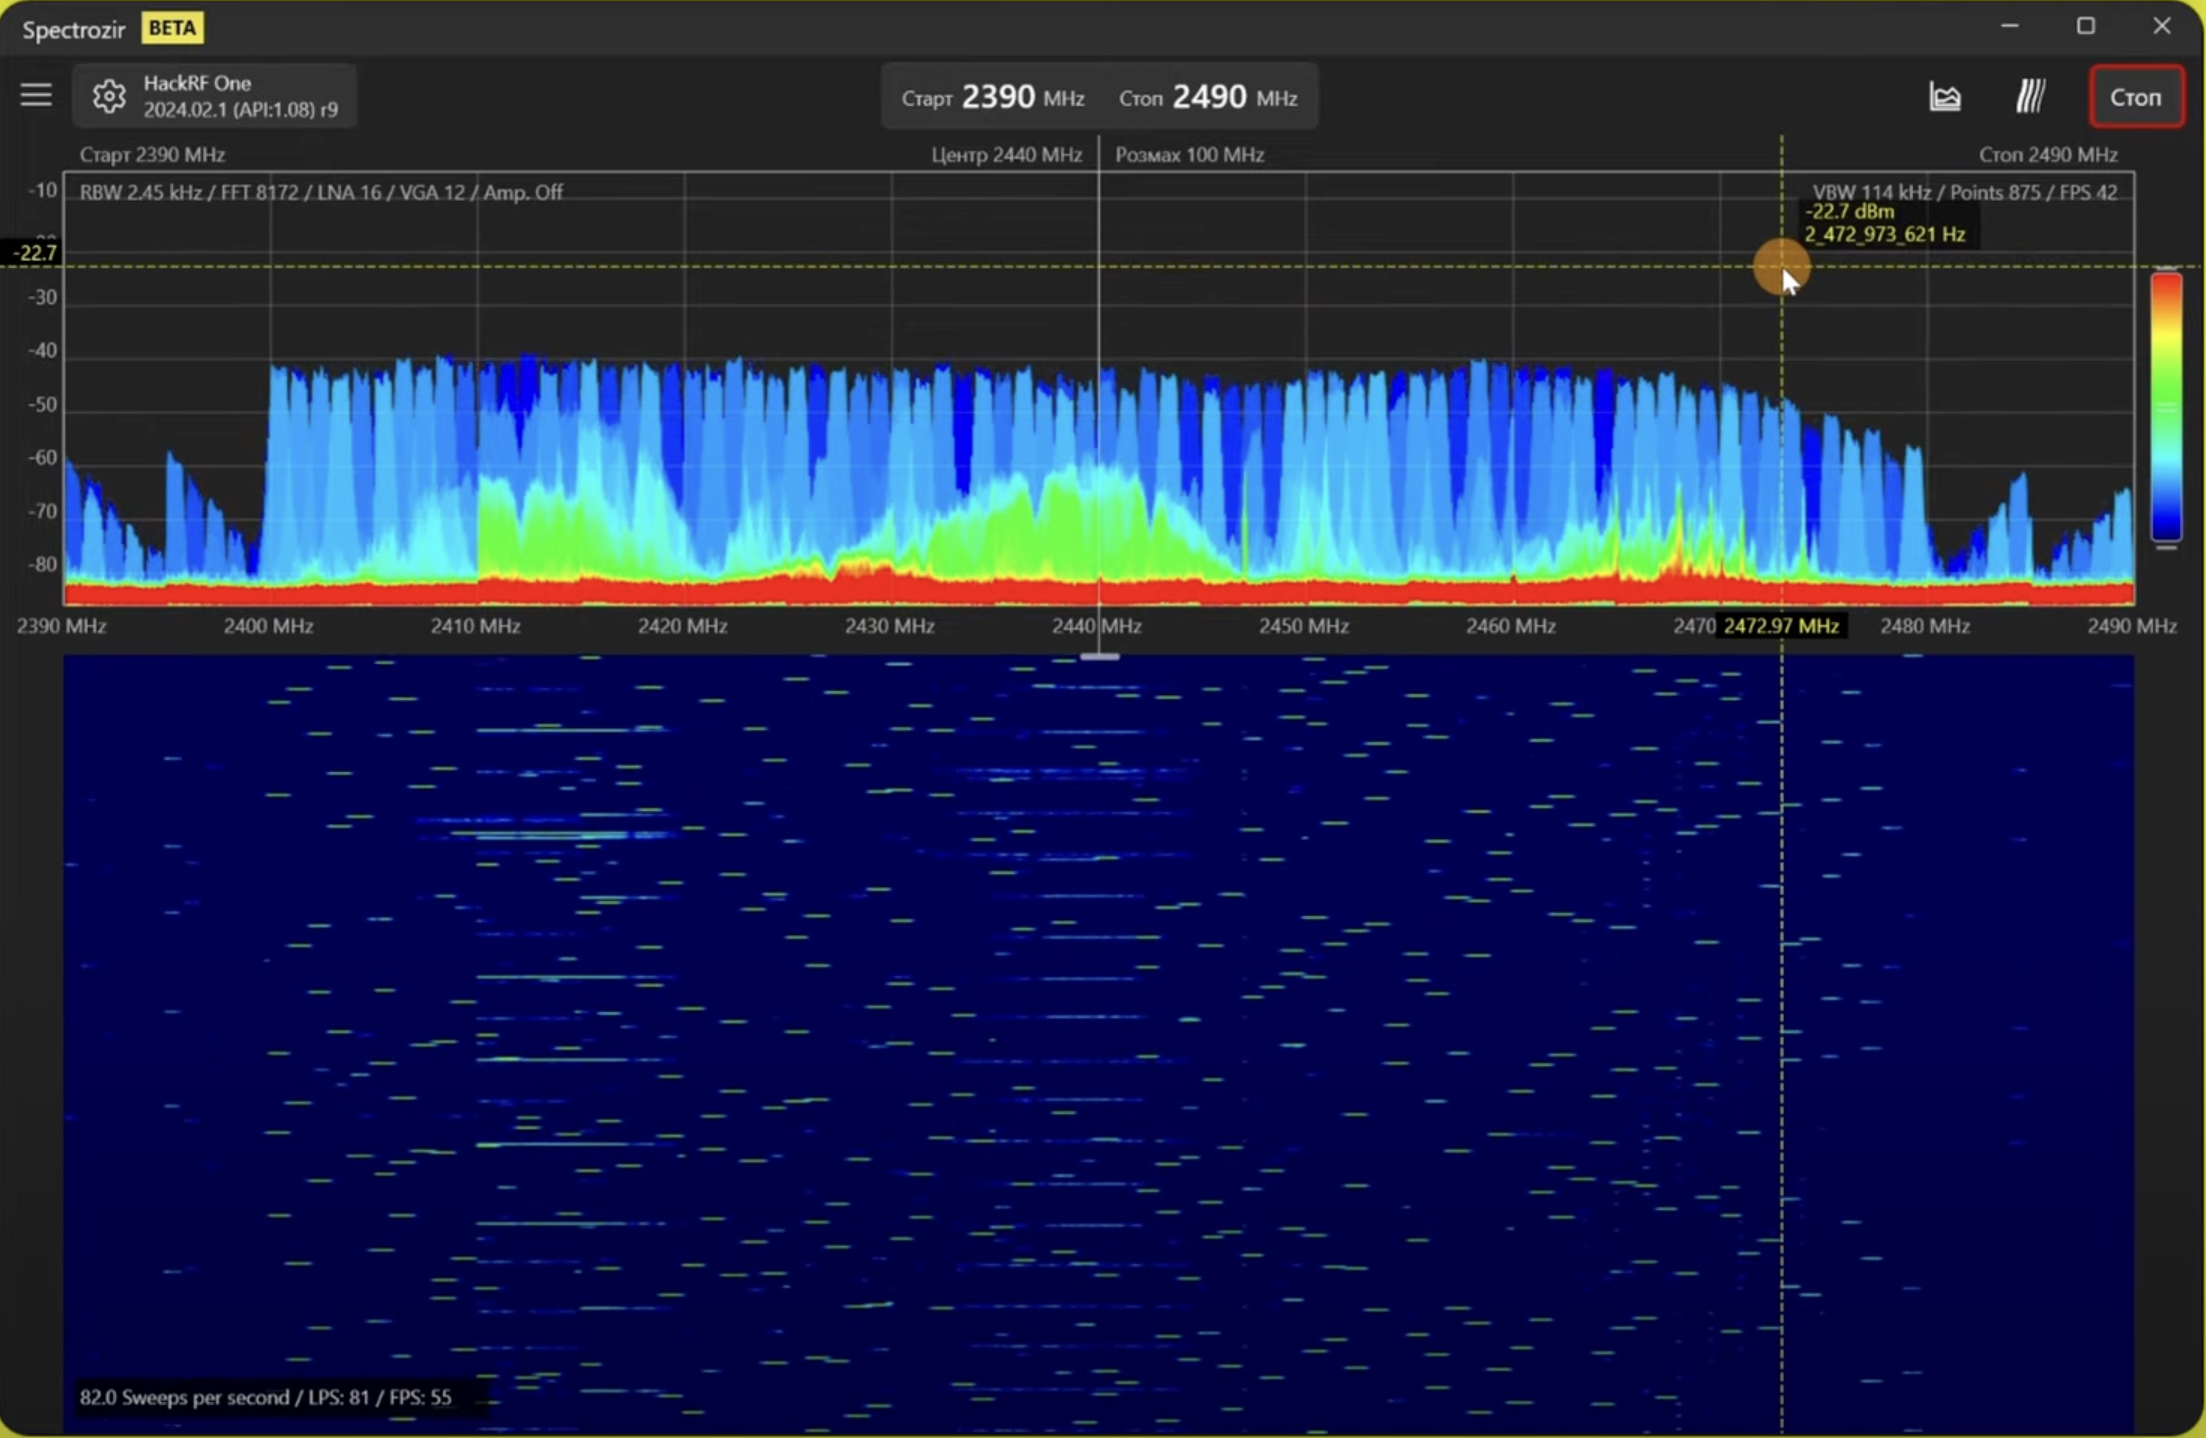
\includegraphics[width=0.7\linewidth]{images/freq-hope.png}
\caption{\label{fig:hf}ППРЧ радіо сигналу протоколу ELRS на частоті 2.4ГГц.}
\end{figure}

Технологія ППРЧ знайшла широке застосування у протоколах керування дронами (сигнал йде від пульта до БПЛА) через властивості такого методу передачі:
\begin{itemize}[noitemsep, topsep=8pt]
\item \textbf{Стійкість до перешкод}: Сигнал на кожній окремій частоті передається протягом короткого періоду часу, що робить його важче заглушити.
\item \textbf{Ефективність спектра}: Покращує ефективність використання радіочастотного спектра, оскільки сигнал розподіляється по різних частотах.
\end{itemize}

Якщо дуже спрощено, то сигнали керування від пульта (фактичні дії оператора) перетворюються на окремі пакети, які передаються по радіоканалах на певній смузі у псевдовипадковому режимі. Для того щоб подавити такий сигнал, потрібно створювати заваду не на окремих каналах передачі, а по всій смузі частот. Більше детально, як виглядає ППРЧ, можна \href{https://www.youtube.com/watch?v=REyNJcrZHII}{подивитись у відео за посиланням}.

\subsection{LORA}
\textbf{LORA} --- це технологія, яка була розроблена для застосувань з великим радіусом дії, низьким енергоспоживанням та низькою швидкістю передачі даних. LORA це саме фізичний рівень, який використовується в LoRaWAN. LoRaWAN визначає протокол зв'язку та системну архітектуру мережі. Технологія працює на основі модуляції чірпу (CSS -  Chirp Spread Spectrum), стійкий до перешкод та багатопроменевих згасань. Чірп розшифровується як «стиснутий високоінтенсивний радіолокаційний імпульс». Це сигнал, частота якого з часом або збільшується, або зменшується. LoRa має 6 (SP - speading factors) коефіцієнтів розсіювання (SF7 - SF12) та три різні пропускні смуги (125 кГц, 250 кГц та 500 кГц). Символи LoRa модулюються по висхідному частотному сигналу смуги  і використовуються різні ортогональні коефіцієнти розширення залежно від вимог до швидкості передачі даних та умов каналу.

\begin{figure}[h!]
	\centering
	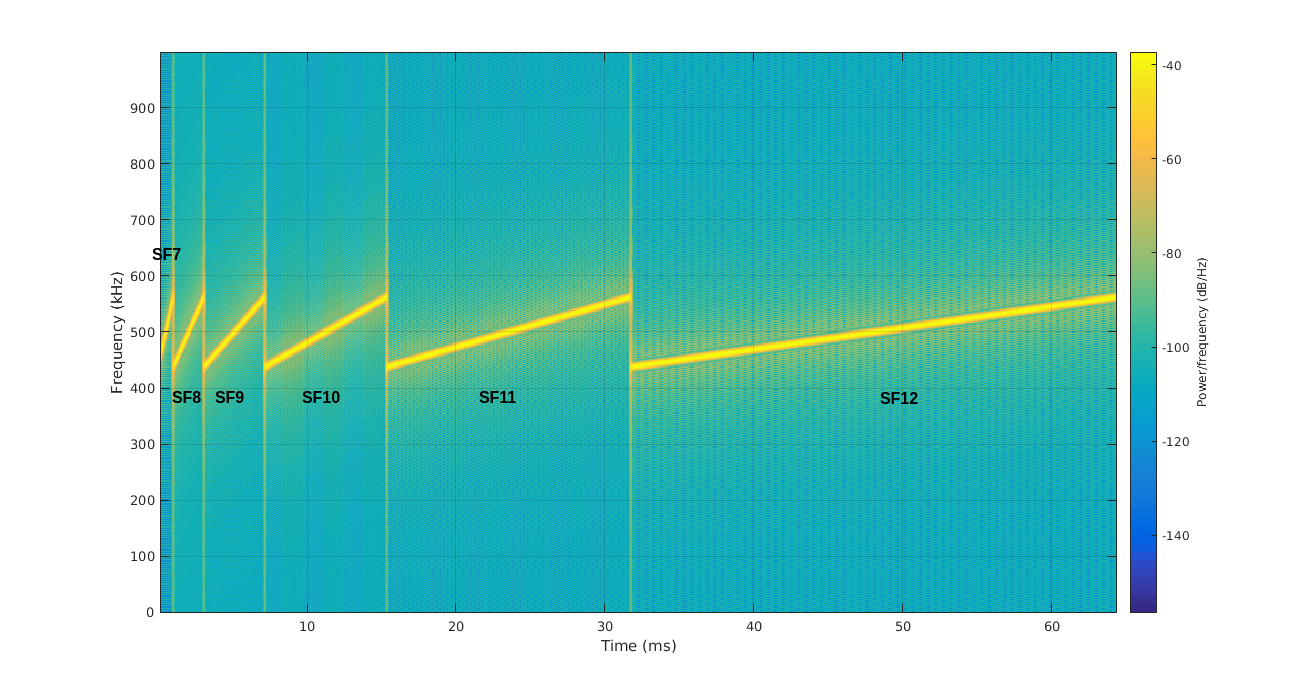
\includegraphics[width=1\linewidth]{images/lora_chirps.png}
	\caption{\label{fig:lora_chirps} Cпектрограма різного спредінг фактору.}
\end{figure}

Фізичний рівень LoRa включає преамбулe, 2 символи синхронізації та корисну інформацію.
Із важливого варто зазначити, що:
\begin{itemize}[noitemsep, topsep=8pt]
\item SF8 займає точно вдвічі більше часу, ніж SF7, а SF9 займає точно вдвічі більше часу, ніж SF8. Співвідношення швидкості передачі символів (Rs), пропускної здатності (BW) та коефіцієнта розширення (SF) визначається за формулою:

\[
R_s = \frac{\mathrm{BW}}{2^{\mathrm{SF}}}
\]
\item Вищий коефіцієнт розширення - Більший час передачі даних.
\item Нижчий коефіцієнт розширення - Вища швидкість передачі даних.
\end{itemize}


\begin{figure}[h!]
	\centering
	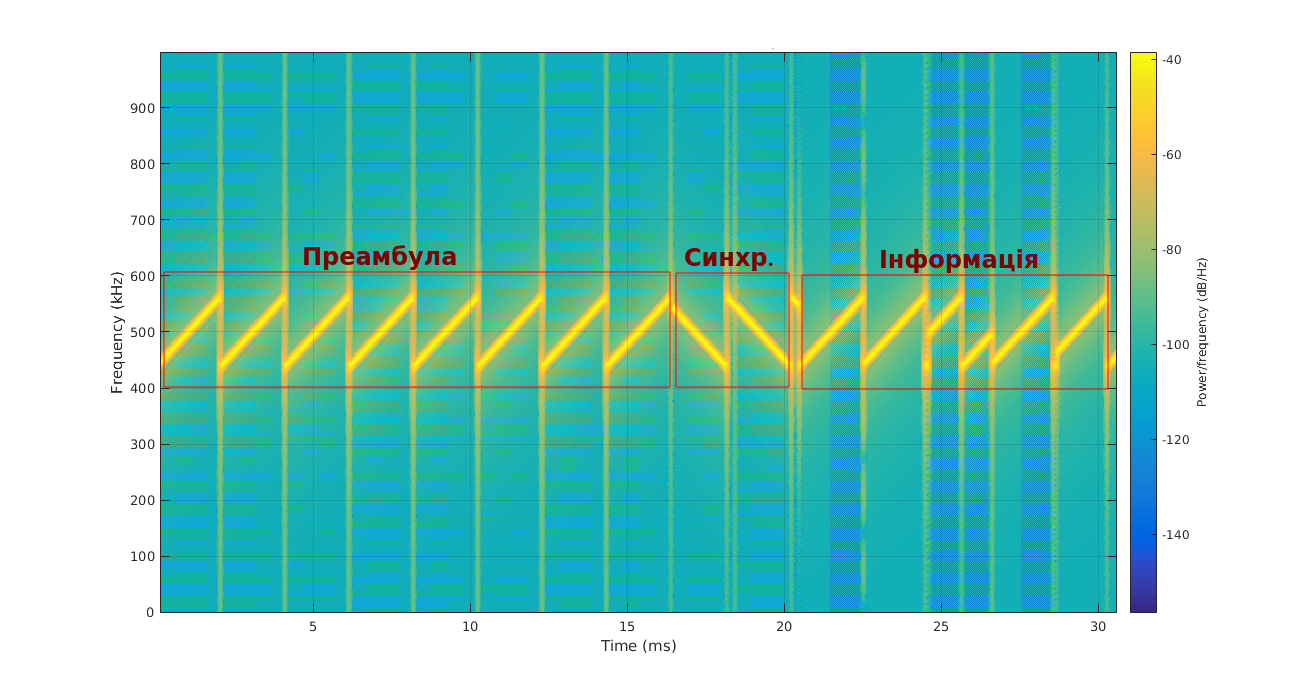
\includegraphics[width=1\linewidth]{images/lora_preambul.png}
	\caption{\label{fig:lora_preambul} Приклад пакету LORA}
\end{figure}

Перші 8 символів підвищеного чирпу – це символи преамбули, що використовуються для виявлення чирпів LoRa, наступні 2 символи зниження чирпу – це символи синхронізації, що використовуються для синхронізації часу, а потім йдуть модульовані символи, тобто корисна інформація. Стрибок частоти представляє модульований символ.


\newpage
\section{Спектральний аналіз}

Щоб зрозуміти, що таке спектральний аналіз, нагадаю про важливі властивості хвиль --- ми можемо взяти декілька сигналів (позначені синім) і просумувати їх в один фінальний сигнал (позначений червоним), тим самим отримавши комплексний сигнал. Таким чином працює модуляція (див. секцію \ref{sec:modulation}).

\begin{figure}[h!]
\centering
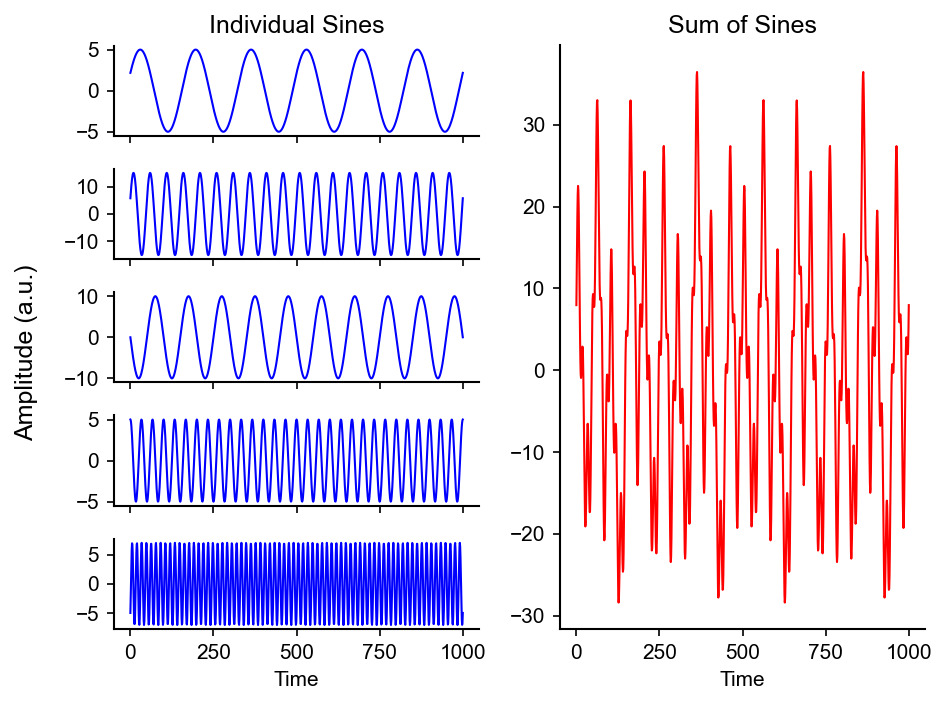
\includegraphics[width=0.6\linewidth]{images/signals-sum.png}
\caption{\label{fig:signals-sum}Процес формування \textit{складного} сигналу шляхом складання декількох окремих сигналів.}
\end{figure}

Цю процедуру можна зробити і в зворотньому напрямку --- отримавши сигнал із радіоефіру, застосовуючи певні алгоритми\footnote{Для розкладання сигналу на складові виконується обробка сигналу під назвою \textit{швидке перетворення Фур'є} (FFT)}, розкласти його на складові. Кожна складова — це синусоїдальний сигнал зі своєю частотою. Таким чином ми можемо відобразити складові на окремому графіку, тим самим відобразивши сигнал у \textbf{частотній області} (або ще можна зустріти термін \textbf{частотний домен}\footnote{Тема частотного домену і перетворення Фур'є дуже цікава, але обширна. Більш поглиблено про це можна почитати в \href{https://pysdr.org/ukraine/content-ukraine/frequency_domain.html}{інших джерелах}.}). На малюнку \ref{fig:freq-domain} частотна область зображена голубим кольором. Цей графік дає нам можливість зрозуміти, які складові присутні у сигналі на певному діапазоні частот.

\begin{figure}[h!]
\centering
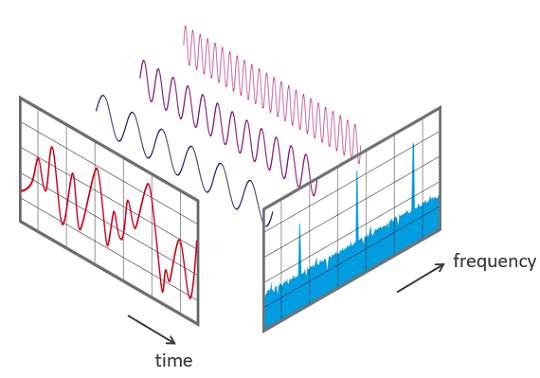
\includegraphics[width=0.7\linewidth]{images/freq-domain.png}
\caption{\label{fig:freq-domain}Розкладання сигналу на складові або перевід сигналу з часової у частотну область.}
\end{figure}

Відображення сигналу у частотній області відповідає певному проміжку часу. Наприклад, ми записуємо сигнал із радіоефіру тривалістю \texttt{0.1c} з діапазоном частот від \texttt{500MГц -- 1ГГц} і будуємо для нього відображення у частотній області. Якщо ми повторимо цю процедуру, скажімо, \texttt{100} разів, то отримаємо \texttt{100} графіків у частотній області, які відповідають одному й тому самому діапазону, але кожен окремо відображає свій проміжок часу. Тепер, якщо ми їх складемо, то отримаємо картину того, як сигнал (а саме його складові) змінювався у часі. Це те, що ми бачимо на екрані спектроаналізатора.

\begin{figure}[h!]
\centering
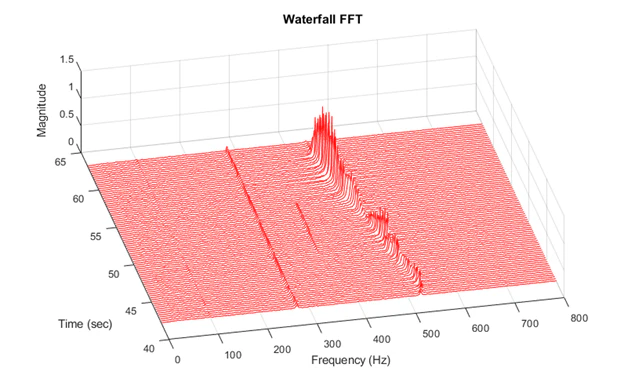
\includegraphics[width=0.75\linewidth]{images/fft-stack.png}
\caption{\label{fig:fft-stack}FFT перетворення складені у стек.}
\end{figure}

Опціонально, можна накласти \textit{тепловий градієнт} на графік, підсвічуючи гарячим області з більшою амплітудою сигналу\footnote{Майже кожен тип модуляції має свій характерний малюнок на водоспаді. Знаючи їх, можна впізнавати сигнали від БПЛА, перевіряти засоби РЕБ (чи працюють вони на заявлених діапазонах і яка щільність завади). Пристрої, за допомогою яких це можна зробити, називаються \textbf{спектроаналізаторами}.}.

\begin{figure}[H]
    \centering
       \begin{minipage}{0.35\textwidth}
        \centering
        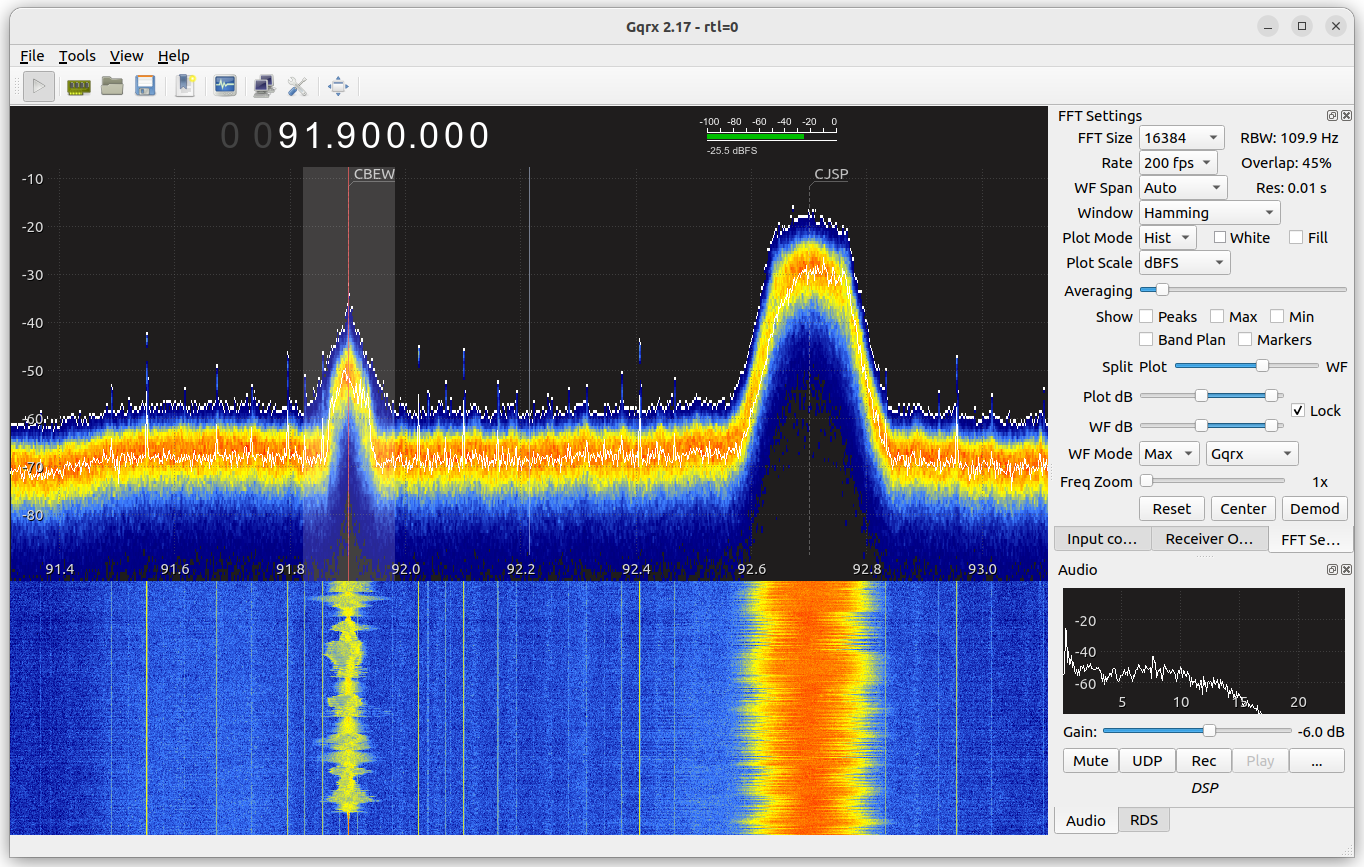
\includegraphics[width=\textwidth]{images/gqrx.png}
    \end{minipage}
    \begin{minipage}{0.55\textwidth}
        \centering
        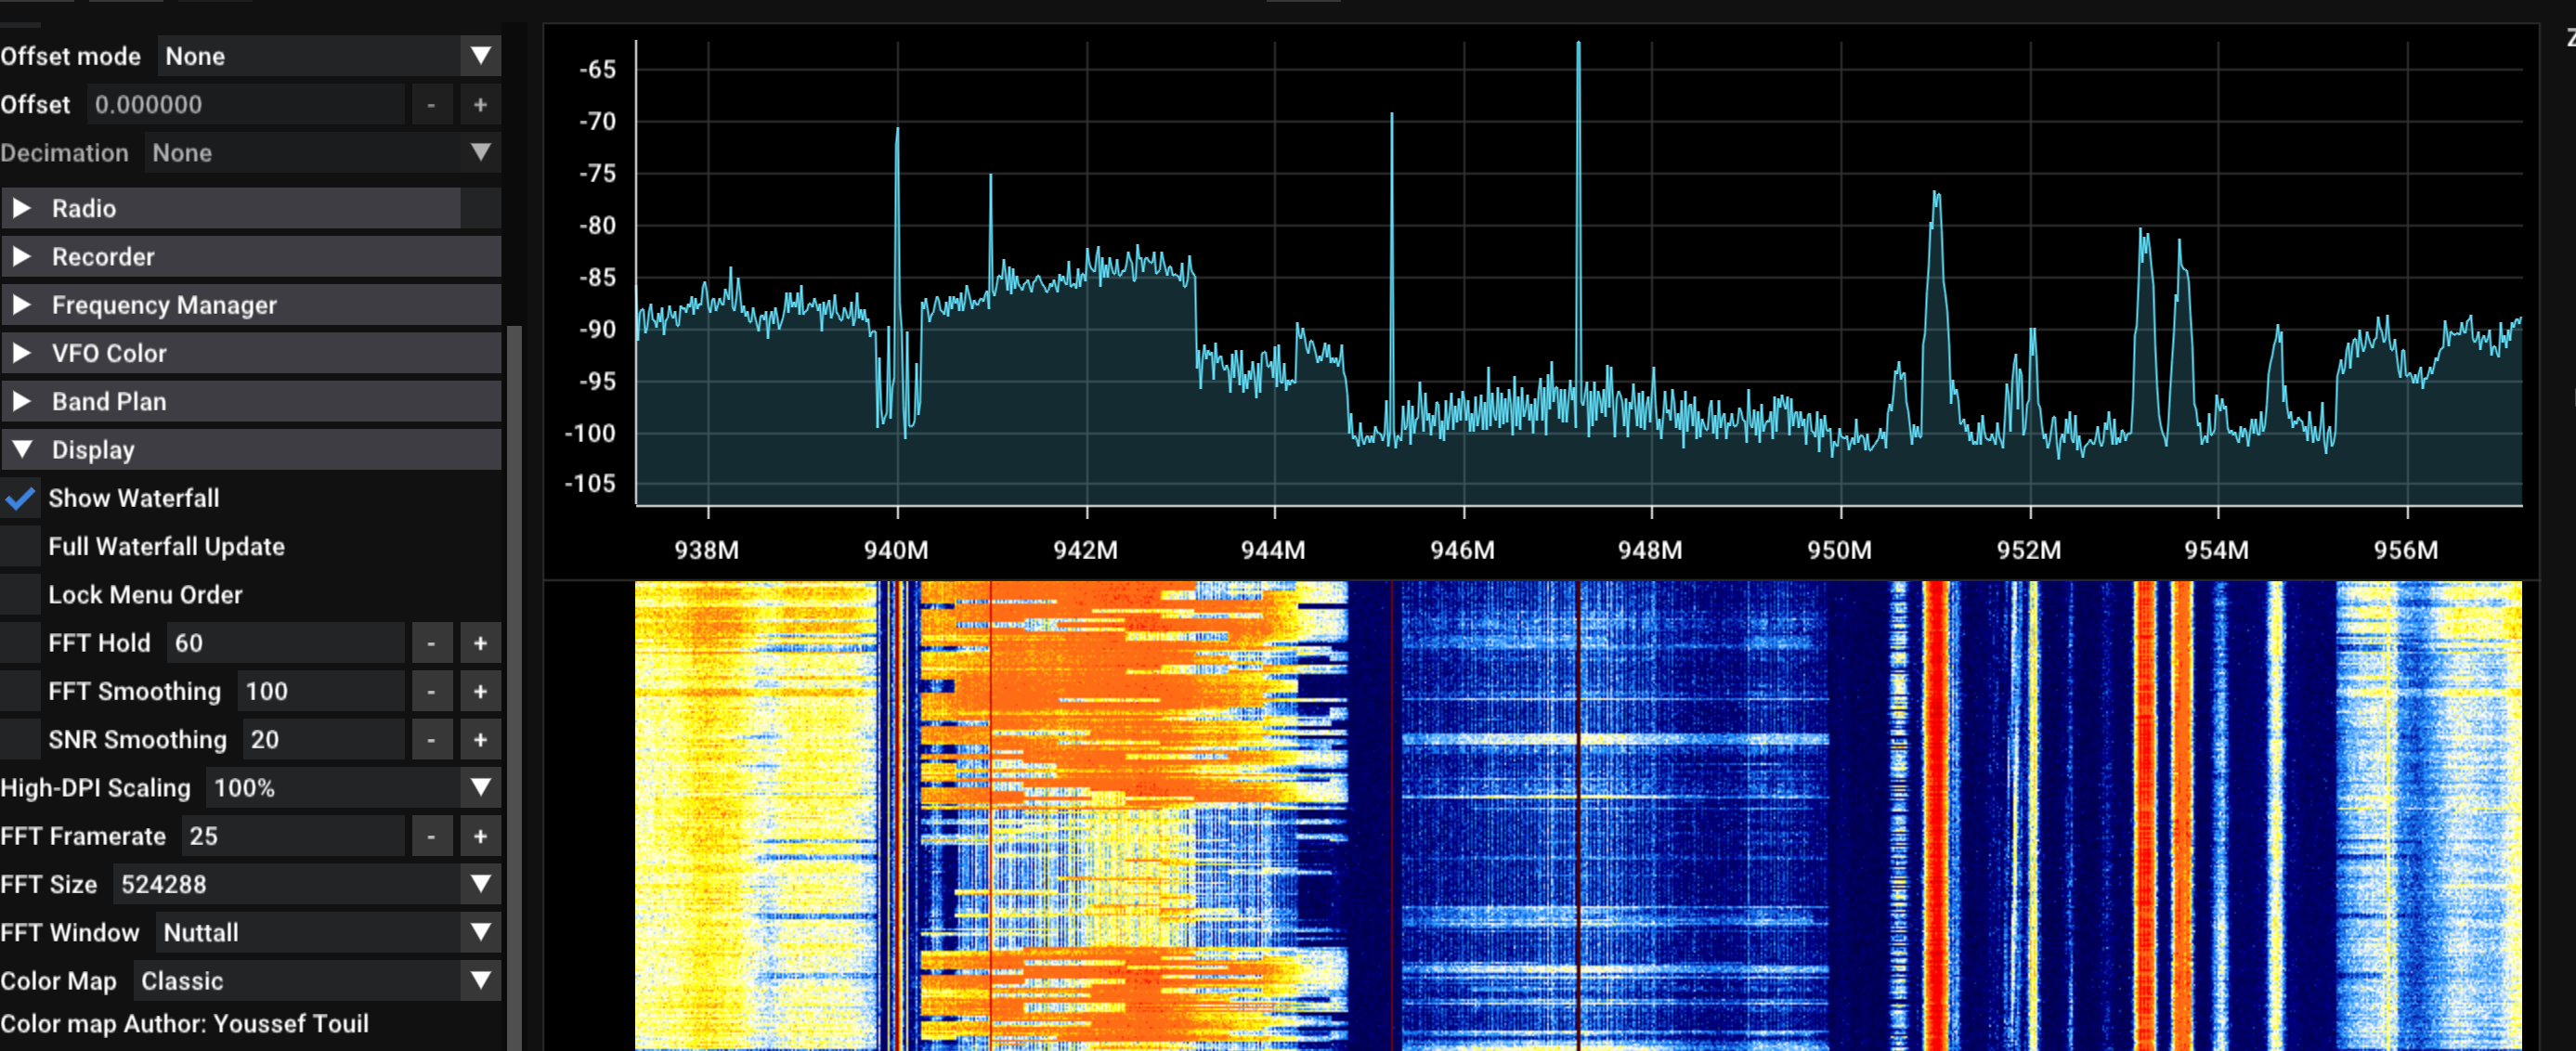
\includegraphics[width=\textwidth]{images/sdrpp.png}
    \end{minipage}
    \caption{Вікно програми GQRX(зліва) і SDR++(справа).}
\end{figure}

\subsection{Обладнання}

Спектроаналізатор --- це тип пристроїв, які мають дуже широку номенклатуру. Вони розрізняються за багатьма параметрами (портативність, частота семплювання, миттєва смуга, розрядність АЦП, тощо), які впливають на вартість приладу. Ціна може починатись від 100\$ і сягати декількох тисяч доларів. В залежності від задачі і бюджету можна підібрати спектроаналізатор під свої потреби.

\begin{figure}[H]
\centering
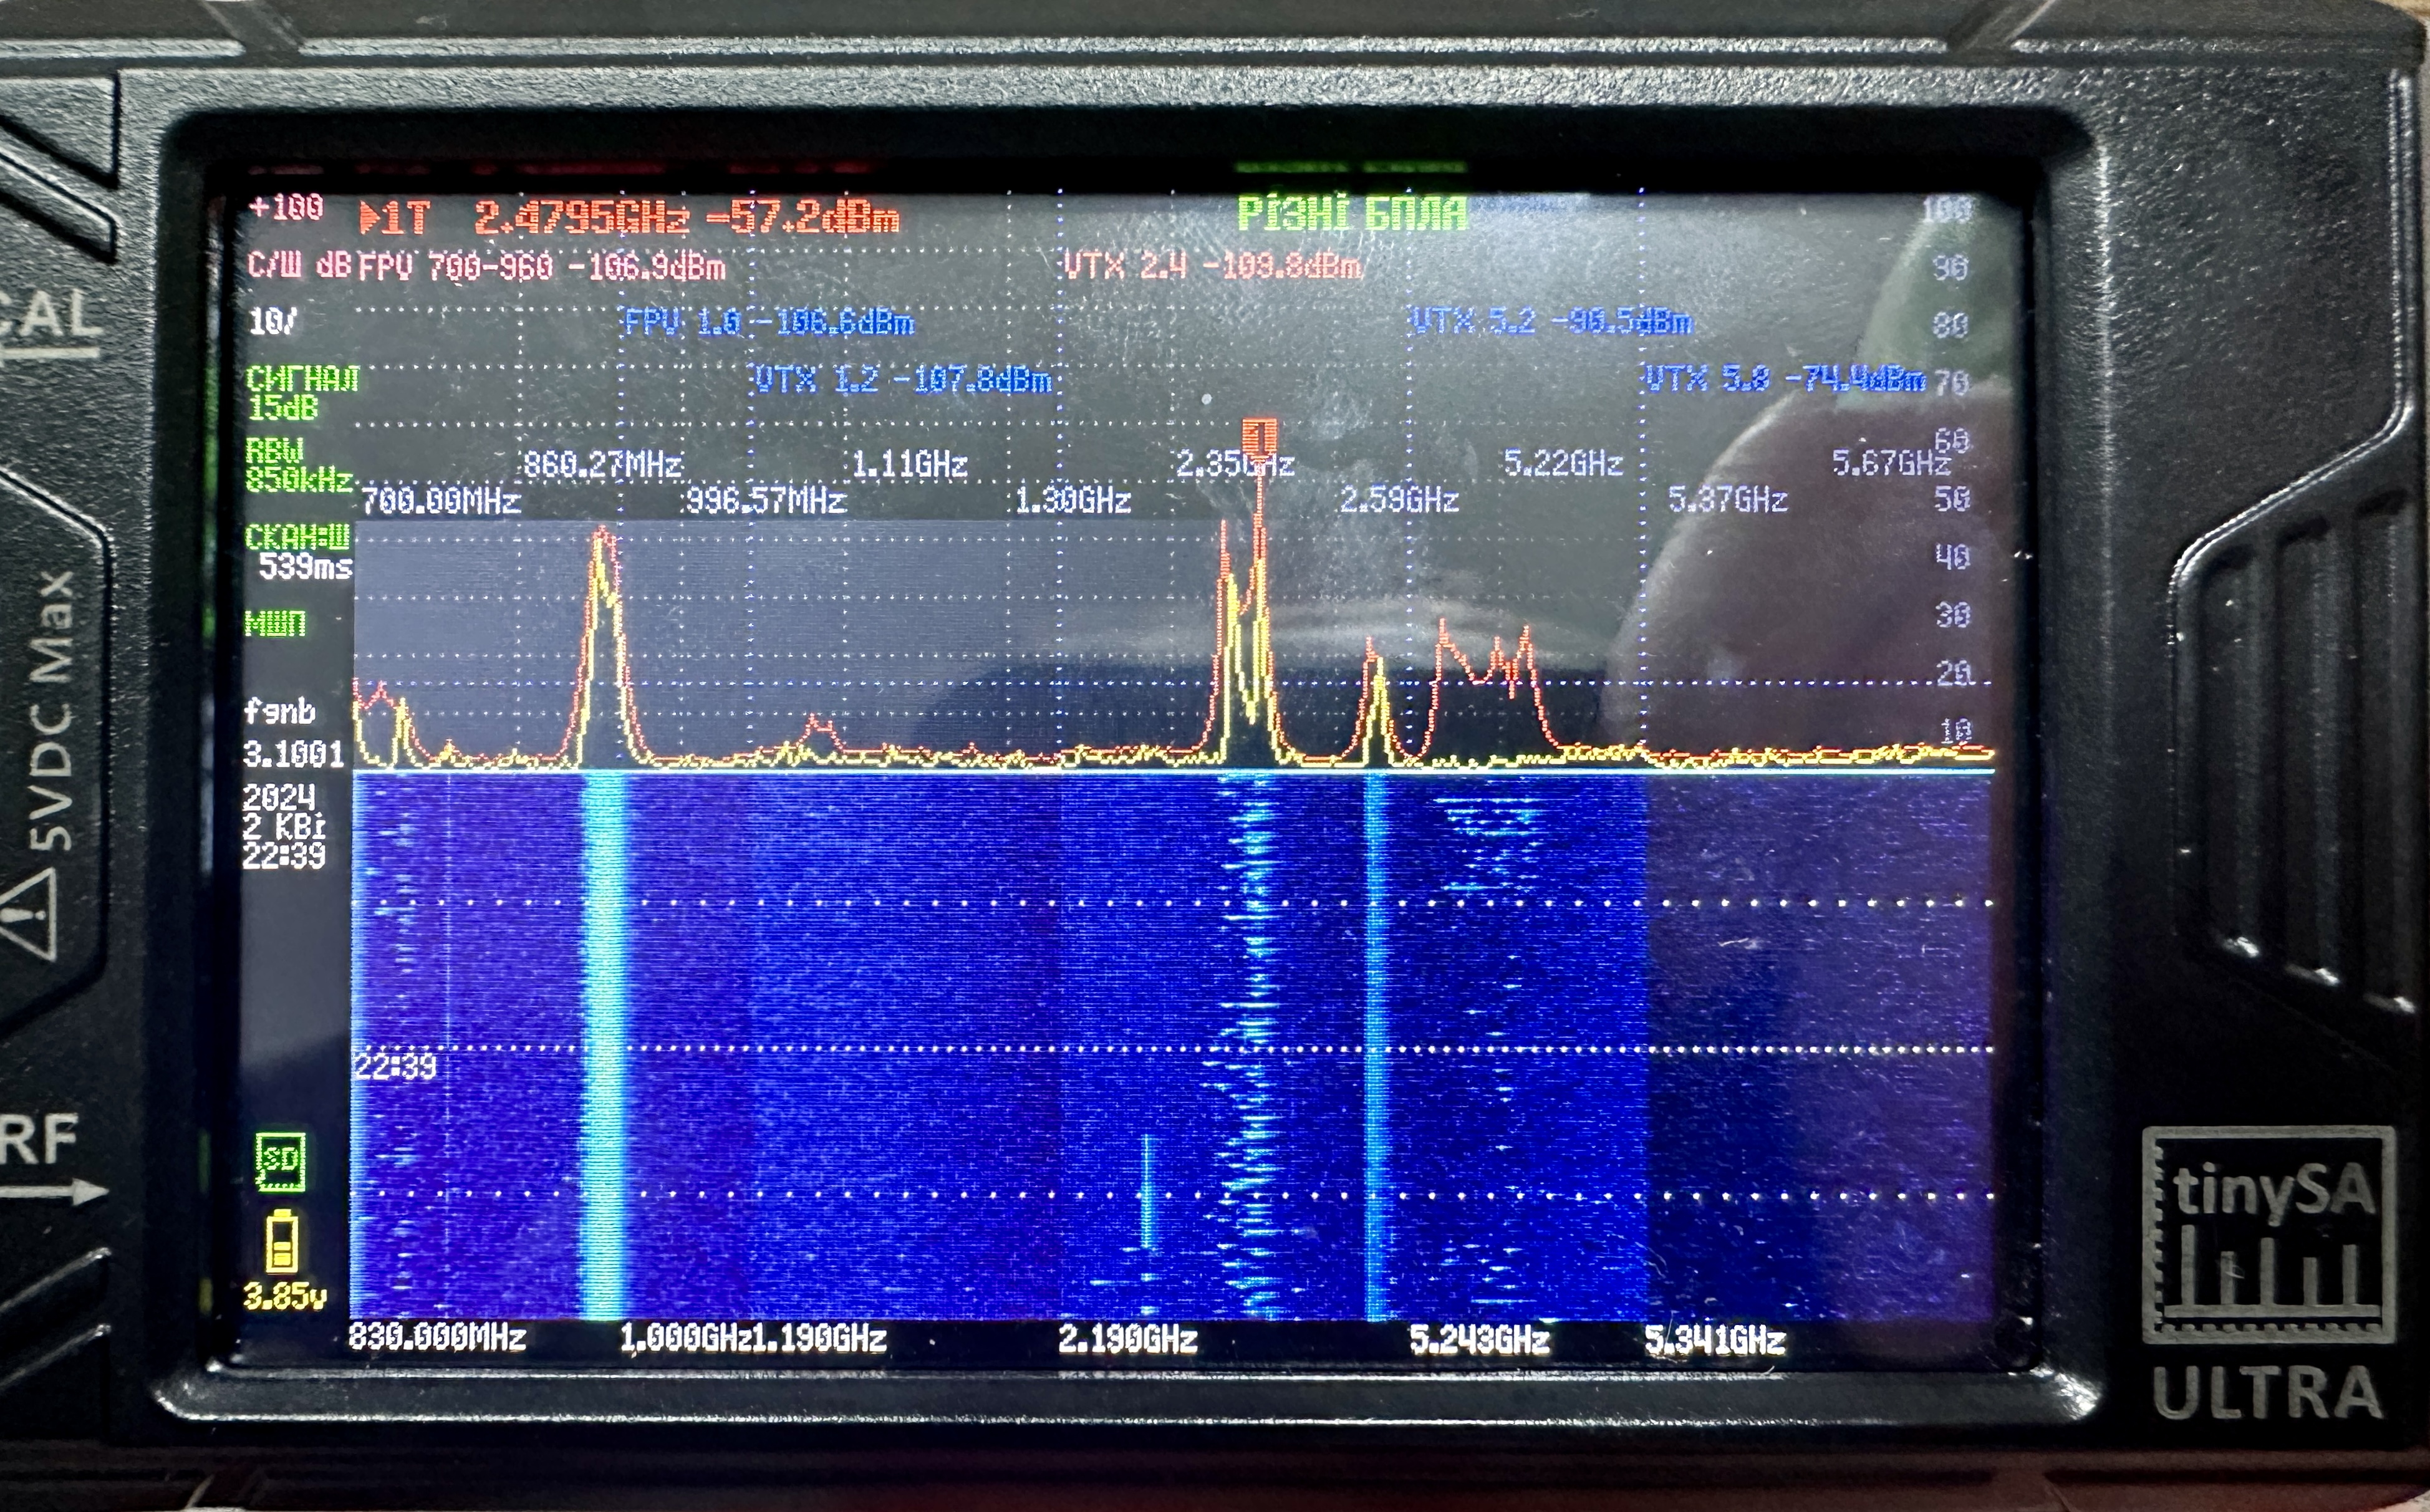
\includegraphics[width=0.7\linewidth]{images/tinysa.jpg}
\caption{\label{fig:tinysa}Портативний спектроаналізатор TinySA Ultra з прошивкою ЗСУ.}
\end{figure}

\textbf{TinySA Ultra} -- портативний спектроаналізатор, який дозволяє робити огляд смуги частот до 6ГГц. Є базові версії і збірки на базі цього пристрою (надрукований корпус на 3D принтері з направленою антеною). Засіб дозволяє:

\begin{itemize}[noitemsep, topsep=8pt]
\item Визначати напрямок сигналу (за допомогою направленої антени), наприклад, відео з FPV дрона.
\item Перевіряти роботу РЕБ шляхом оцінки завади, яка відображається на екрані пристрою.
\item Робити оцінку радіоефіру для розрахунків БпАК (дивитись, які частоти зайняті, щоб уникати перешкод).
\end{itemize}


\textbf{HackRF One} --- це інший клас пристрою початкового рівня, т.н. SDR-приймач. Робочий діапазон також складає до 6ГГц. За допомогою цього засобу можна вирішувати більш складні задачі аналізу, організовувати пост спостереження, записувати т.н. IQ-семпли (дані радіоефіру) для подальшої обробки. Важливо зауважити, що це не пристрій сам в собі, а те, що підключається до робочої станції і потребує додаткового програмного забезпечення\footnote{Перевагою HackRF One є те, що існує багато програмного забезпечення, яке підтримує роботу з цим пристроєм, найбільш відомі: \href{https://airspy.com/download/}{SDR\#}, \href{https://www.sdrpp.org/}{SDR++}, \href{https://www.gqrx.dk/}{GQRX}, \href{https://spectrozir.com/}{Spectorzir}}.

\begin{figure}[H]
    \centering
       \begin{minipage}{0.4\textwidth}
        \centering
        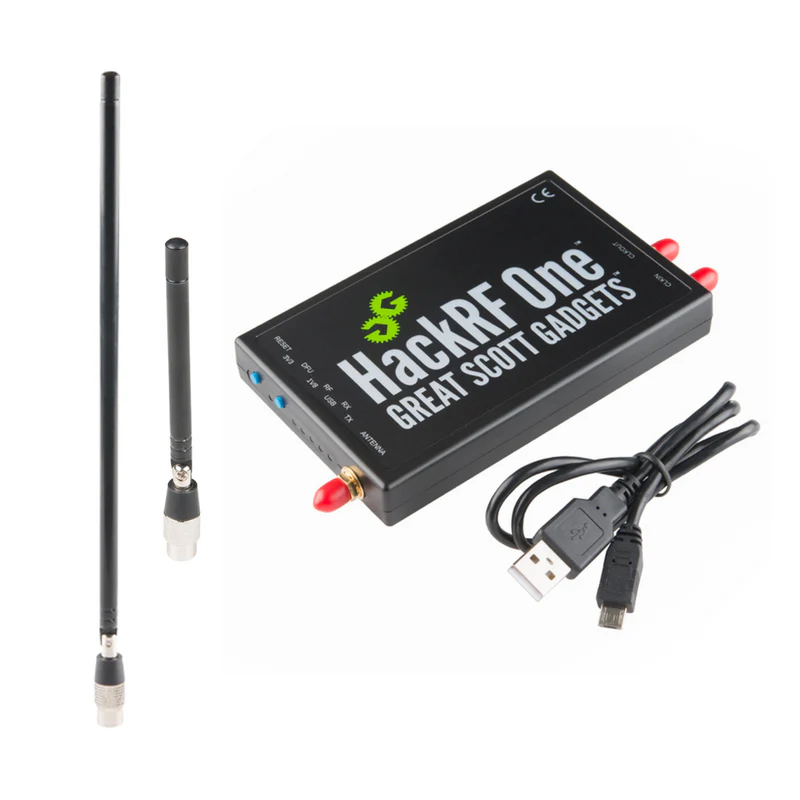
\includegraphics[width=\textwidth]{images/hackrf.png}
    \end{minipage}
    \begin{minipage}{0.3\textwidth}
        \centering
        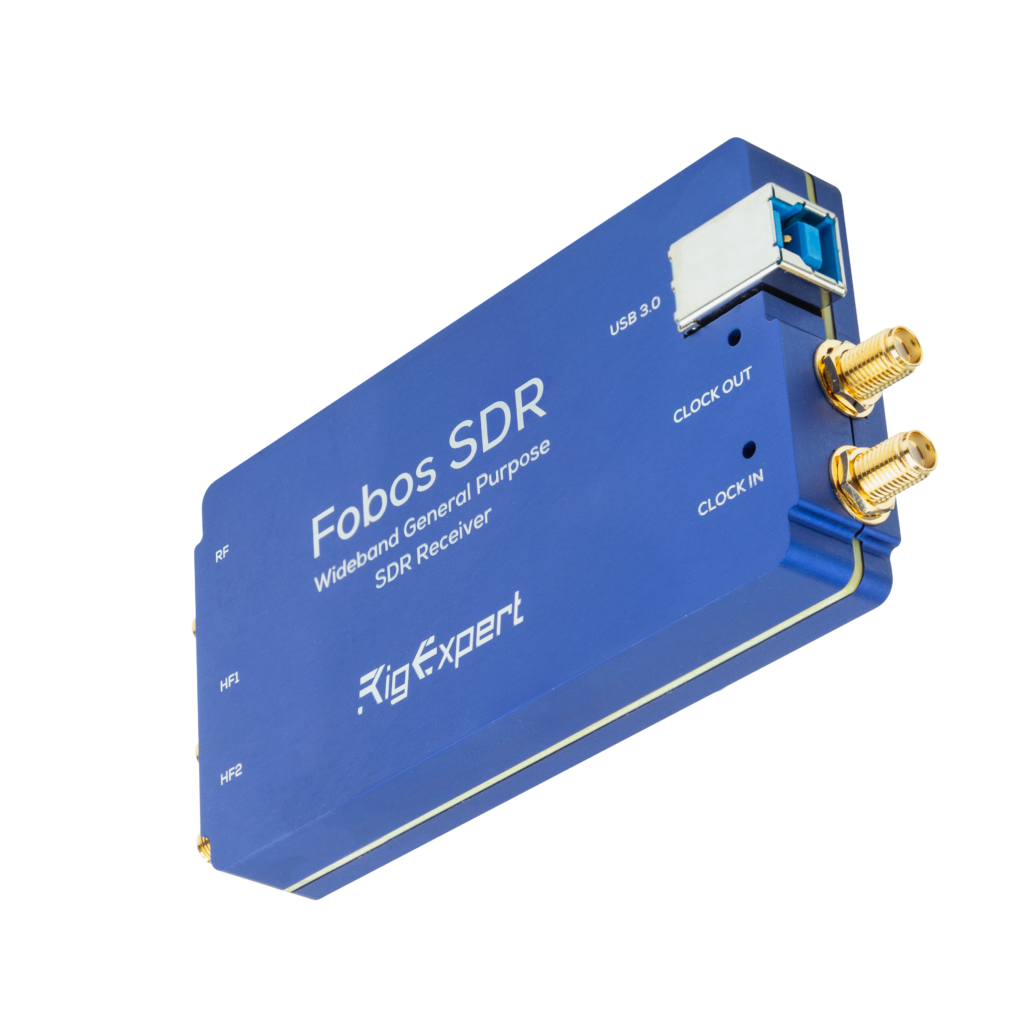
\includegraphics[width=\textwidth]{images/fobos.png}
    \end{minipage}
    \caption{\label{fig:hackrf}Загальний HackrRF One(зліва) і FobosSDR(зправа).}
\end{figure}

\subsection{Додаткові матеріали по темі}

\begin{itemize}[noitemsep, topsep=8pt]
\item \href{https://sprotyvg7.com.ua/lesson/sistemi-radiozvyazku-z-pprch}{Системи радіозв'язку з псевдовипадковим переналаштуванням робочої частоти}.
\item \href{https://www.youtube.com/watch?v=KCj1-SM9aAA}{Порівняння TinySA Base, TinySA Ultra, SA6 (Arinst) та HackRF One}.
\item \href{https://www.youtube.com/watch?v=eFXym8-Yzt0}{Спектр керування FPV на ELRS 915 МГц, знято в екранованій камері на PR200}.
\item \href{https://www.youtube.com/watch?v=REyNJcrZHII}{ELRS 2.4GHz. Як виглядає ППРЧ сигнал радіо протоколу ELRS на частоті 2.4GHz}.
\item \href{https://www.youtube.com/watch?v=XzFMRYEYVXM}{Як виглядає відеосигнал FPV дрона на частоті 5.8 ГГц}.
\end{itemize}

\section{Антени}
\textbf{Антена} --- це пристрій, призначений для передачі або прийому електромагнітних хвиль. Вона перетворює електричні сигнали в радіохвилі при передачі, і радіохвилі в електричні сигнали при прийомі. Далі по тексту, коли буде зустрічатися термін антена, то мається на увазі антена для РЕБ-у. Для РЕБ-у ближньої дії можуть бути використані антени двох типів:

\begin{itemize}[noitemsep, topsep=8pt]
\item \textbf{Направлені} -- мають бути зорієнтовані у напрямку ймовірного маршруту БПЛА.
\item \textbf{Всеспрямовані} -- утворюють т.н. купол навколо засобу РЕБ.
\end{itemize}

\subsection{Діаграма спрямованості}
Антена, що випромінює енергію однаково в усіх напрямках, називається сферичним випромінювачем або ізотропним випромінювачем. Пояснення цього поняття: якщо помістити точкове джерело світла в центр скляної кулі, то її поверхня буде рівномірно освітлена цим джерелом, тобто щільність випромінювання буде однаковою в будь-якій точці поверхні сфери. Однак неможливо створити строго сферичний випромінювач. Він існує лише в теорії і слугує для порівняльних цілей. Жодна реальна антена не здатна забезпечити однакову щільність і поляризацію випромінювання в усіх напрямках. Тому будь-яка антена має певну спрямованість, що описується відповідною діаграмою. Для точного відображення спрямованості необхідно побудувати її тривимірне (просторове) зображення. Однак просторовий розподіл щільності важко відобразити графічно, тому зазвичай обмежуються представленням діаграми спрямованості антени у вертикальній та горизонтальній площинах.

\begin{figure}[H]
\centering
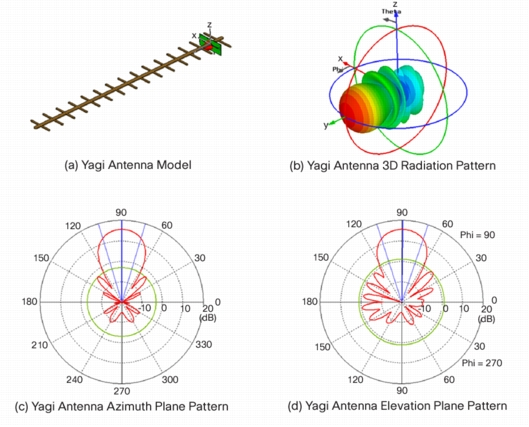
\includegraphics[width=0.6\linewidth]{images/yagi-antenna.jpg}
\caption{\label{fig:yagi:antenna}Діаграма спрямованості з вузькою діаграмою спрямованості.}
\end{figure}

Діаграма спрямованості та підсилення антени взаємопов'язані. Пояснимо їх взаємозв'язок на прикладі скляної кулі. Якщо джерело світла в центрі кулі забезпечити відбивачем (наприклад, параболічним дзеркалом), світло буде йти у вигляді пучка, і випромінювання стане спрямованим. Таким чином, освітленою виявиться лише частина поверхні кулі, обмежена через спрямованість випромінювання. При цьому щільність потоку енергії випромінювання в межах спрямовано освітленої частини поверхні значно перевищить відповідне значення при рівномірному освітленні кулі, оскільки на дану ділянку потраплять також ті промені, які до появи відбивача освітлювали інші частини поверхні. Щільність потоку енергії випромінювання тим вища, чим гостріша спрямованість випромінювання. Тому підсилення за щільністю потоку енергії відносно ізотропного випромінювання прямо залежить від діаграми спрямованості. Як підсилення, так і діаграма спрямованості виражають \textbf{концентрацію випромінювання в певному напрямку}.

\begin{figure}[H]
\centering
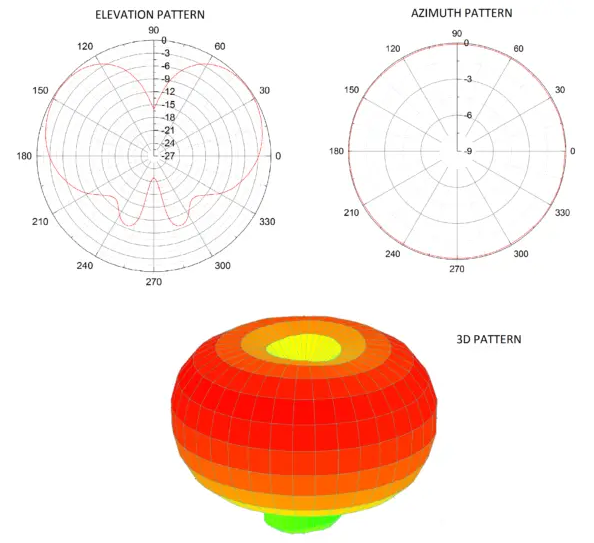
\includegraphics[width=0.5\linewidth]{images/omni-antenna.png}
\caption{\label{fig:omni:antenna}Діаграма спрямованості антени з круговою поляризацією.}
\end{figure}

\subsection{Поляризація антен}

Для електромагнітної хвилі поляризація фактично є площиною, в якій електрична хвиля вібрує. Це важливо при розгляді антен, оскільки вони чутливі до поляризації і зазвичай приймають або передають сигнал лише з певною поляризацією.

Для більшості антен дуже легко визначити поляризацію. Вона просто знаходиться в тій же площині, що і елементи антени. Отже, вертикальна антена (тобто антена з вертикальними елементами) найкраще буде приймати вертикально поляризовані сигнали, а також горизонтальна антена буде приймати горизонтально поляризовані сигнали.

Відповідно, поляризація антен, розташованих у вільному просторі, дуже важлива, і, очевидно, вони повинні знаходитися в однаковій площині, щоб забезпечити оптимальний сигнал. Якби вони знаходились під прямим кутом один до одного (тобто крос-поляризовані), то теоретично сигнал не приймався б, але на практиці, коли у антен (засобу подавлення і на дроні) різні поляризації, то такий засіб \textbf{працювати буде}, але із втратою ефективності (див. Табл. \ref{table:polarization}).

\begin{table}[ht]
\centering
\begin{tabular}{|l|l|l|l|l|l|}
\hline
\textbf{Поляризація / Db} & \textbf{Верт.} & \textbf{Гор.} & \textbf{Під 45°} & \textbf{Право кругова} & \textbf{Ліво кругова} \\
\hline
Вертикальна      & 0           & $\infty$     & 3            & 3            & 3            \\
Горизонтальна    & $\infty$    & 0            & 3            & 3            & 3            \\
Під 45°          & 3           & 3            & 0 або $\infty$ & 3            & 3          \\
Право кругова    & 3           & 3            & 3            & 0            & 3            \\
Ліво кругова     & 3           & 3            & 3            & 3            & 0            \\
\hline
\end{tabular}
\caption{\label{table:polarization}Вплив розташування антен з різним типом поляризації \cite{book:rothammel}.}
\end{table}


\textbf{Приклади}. Для дрона з горизонтальною антеною (горизонтальна поляризація) і засобом подавлення з вертикальною антеною (вертикальна поляризація) типу діполь (штирьова антена) подавлення буде неефективним. Для цього на практиці такого типу антени намагаються розташувати під кутом 45 градусів. Тому виробники якісного РЕБ-у встановлюють антени типу \textit{конюшина}, \textit{діск-конусні}, \textit{квадрифилярні}, тощо, які дають складну поляризацію.

\begin{figure}[H]
\centering
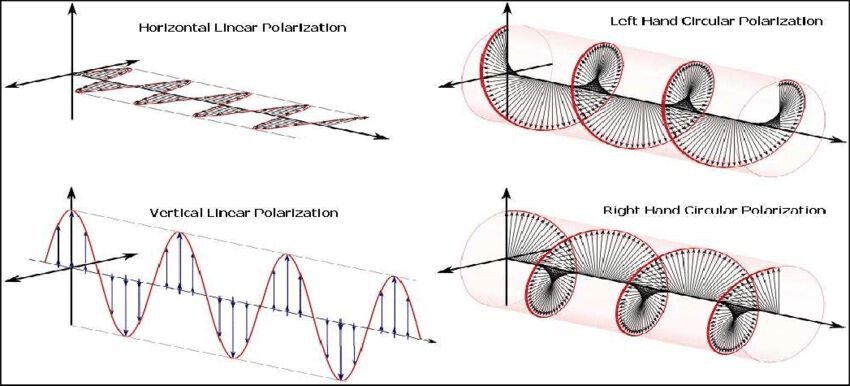
\includegraphics[width=0.7\linewidth]{images/polarization.jpeg}
\caption{\label{fig:polarization}Основні типи поляризацій антен.}
\end{figure}

\subsection{Хвильовий опір антени}
Опір антени, або хвильовий опір антени, це характеристичний параметр антени, який описує, як антена передає або приймає електромагнітні хвилі. Він визначає, як електричні сигнали, що передаються через антену, перетворюються на радіохвилі, і навпаки, як радіохвилі, що приймаються антеною, перетворюються на електричні сигнали. Опір антени складається з двох основних компонентів:

\begin{itemize}[noitemsep, topsep=8pt]
\item \textbf{Активний опір} (омічний опір) --- це частина опору, яка відповідає за перетворення електричної енергії в радіохвилі (випромінювання). Активний опір сприяє випромінюванню сигналу в навколишній простір.
\item \textbf{Реактивний опір} --- це частина опору, яка відповідає за зберігання енергії в електричному або магнітному полях навколо антени. Реактивний опір не сприяє випромінюванню енергії, але може призводити до її втрат у вигляді тепла.
\end{itemize}

Хвильовий опір антени важливий для забезпечення максимальної ефективності передачі енергії від передавача до антени або від антени до приймача. Щоб уникнути відбиття сигналів і забезпечити максимальне випромінювання або прийом сигналу, необхідно, щоб опір антени був узгоджений з хвильовим опором фідера (кабеля), що підключений до антени. Це узгодження відбувається, коли імпеданс (загальний опір) антени дорівнює імпедансу фідера.


\begin{figure}[H]
\centering
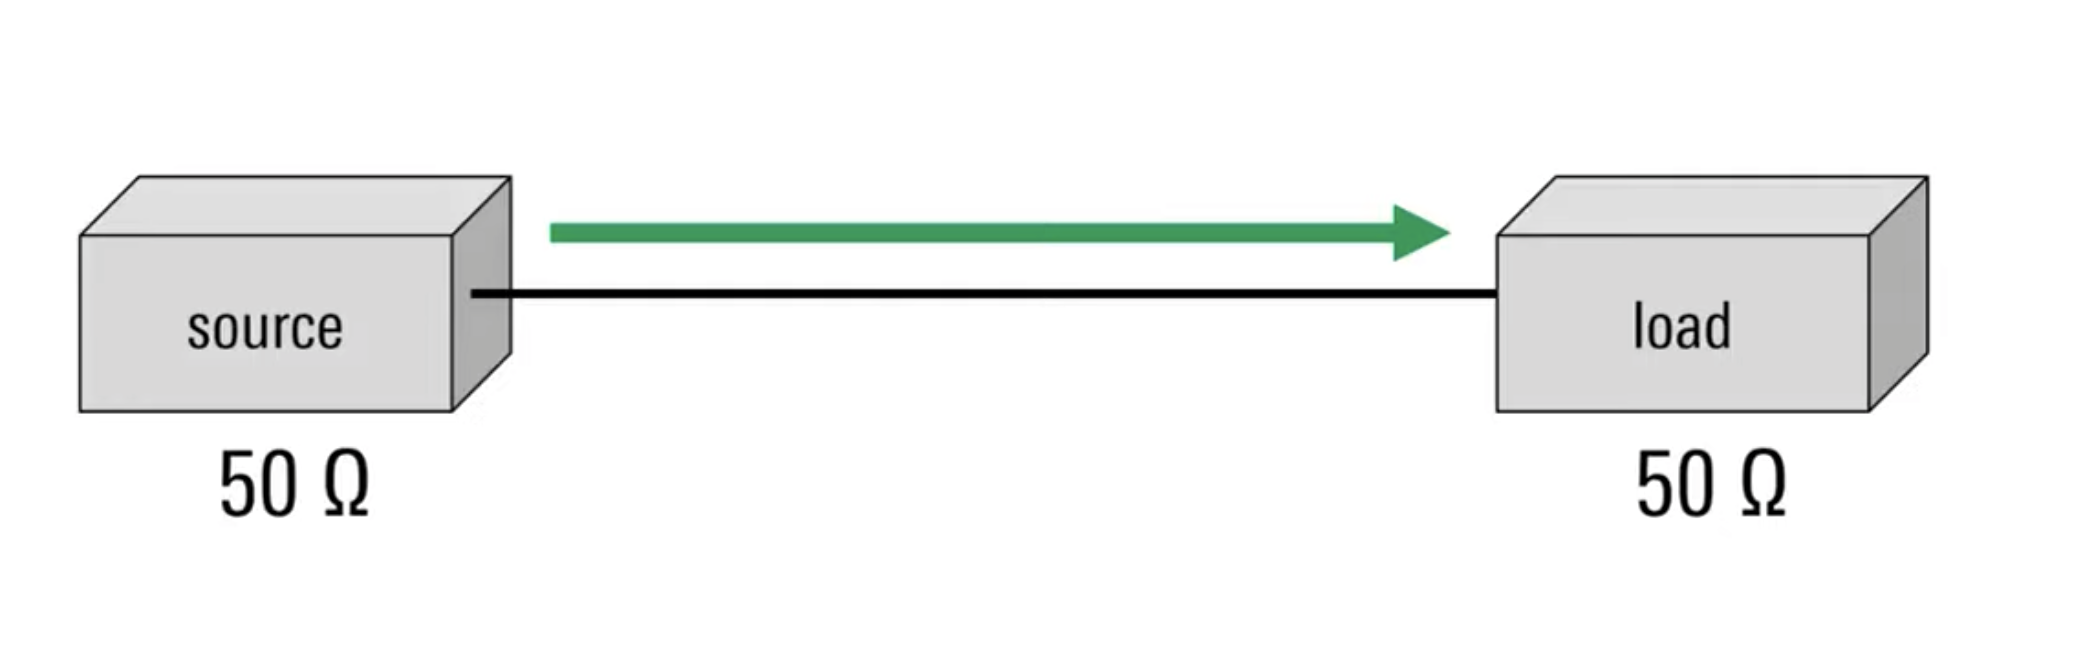
\includegraphics[width=0.75\linewidth]{images/impedance.png}
\caption{\label{fig:impedance}Узгоджений хвильовий опір.}
\end{figure}

\textbf{Важливо!} Опір антени — це величина, яка залежить від частоти.

\subsection{Зворотні втрати антени}

\textbf{Зворотні втрати} антени (англ. \textit{Return Loss}) --- це параметр, який описує, наскільки добре хвильовий опір антени узгоджений з хвильовим опором передавального або приймального тракту (кабеля). Це міра відбитої енергії від антени назад до джерела сигналу через невідповідність імпедансу між антеною і кабелем.

\begin{itemize}[noitemsep, topsep=8pt]
\item \textbf{Зворотні втрати} вимірюються в децибелах (дБ) і позначають різницю потужності, яка подається на антену, і яка відбилася від антени.
\item Високі значення зворотних втрат свідчать про те, що більша частина енергії передається через антену і лише незначна частина відбивається назад. Це є бажаним для оптимальної роботи системи.
\item Низькі значення зворотних втрат означають, що значна частина енергії відбивається назад до джерела сигналу, що свідчить про погане узгодження імпедансів і може призводити до втрат сигналу та зниження ефективності роботи антени.
\end{itemize}

\begin{figure}[H]
\centering
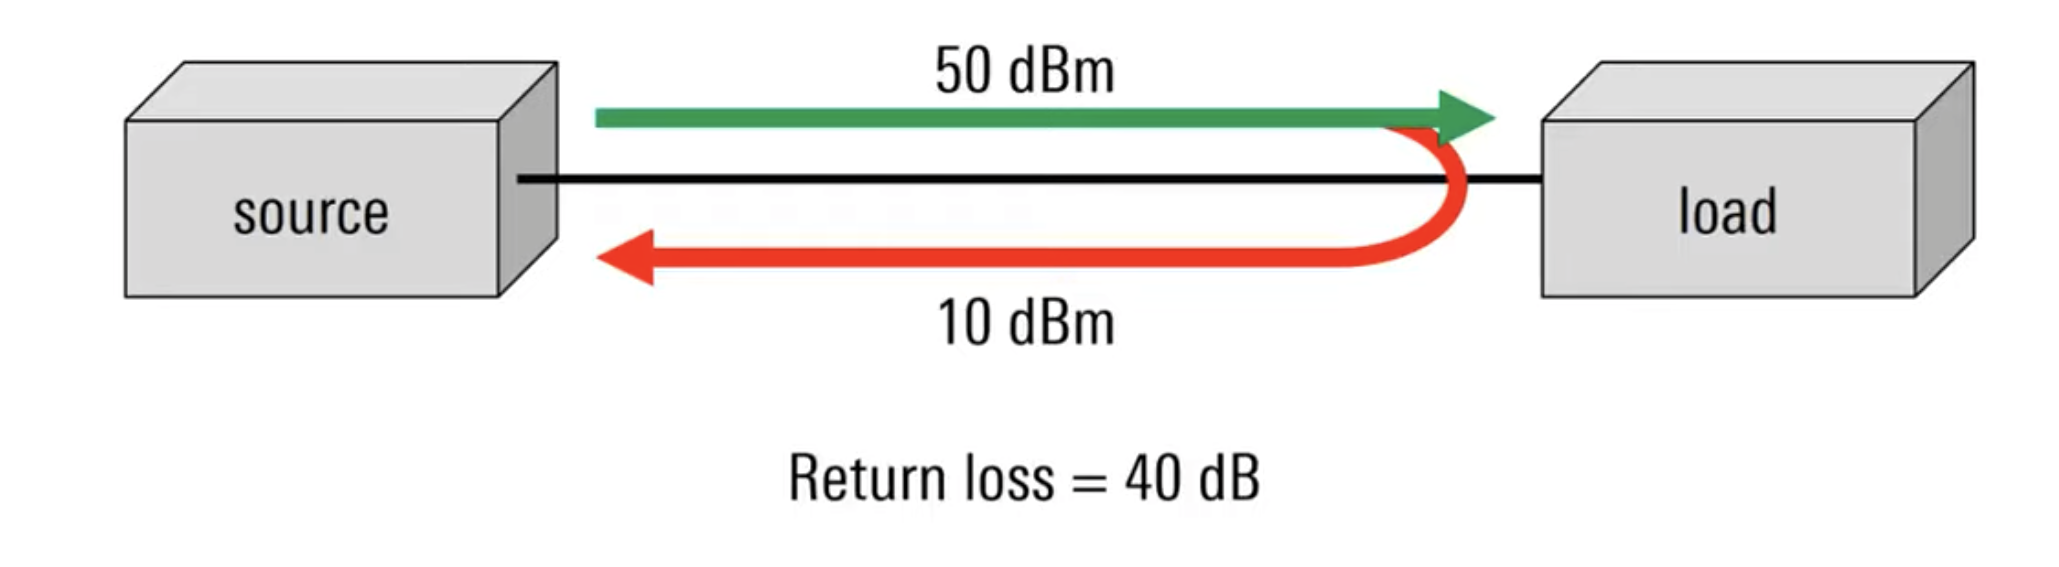
\includegraphics[width=0.75\linewidth]{images/return-loss.png}
\caption{\label{fig:return-loss}Зворотні втрати антени.}
\end{figure}

\subsection{КСХ антени}
\textbf{КСХ} (коефіцієнт стоячої хвилі, VSWR, SWR) антени — це параметр, який показує, наскільки добре антена узгоджена з хвильовим опором фідера (кабеля), до якого вона підключена. КСХ (англійською VSWR — Voltage Standing Wave Ratio) вказує на відносний рівень стоячих хвиль, що утворюються через невідповідність імпедансів антени і кабеля.

\begin{figure}[H]
\centering
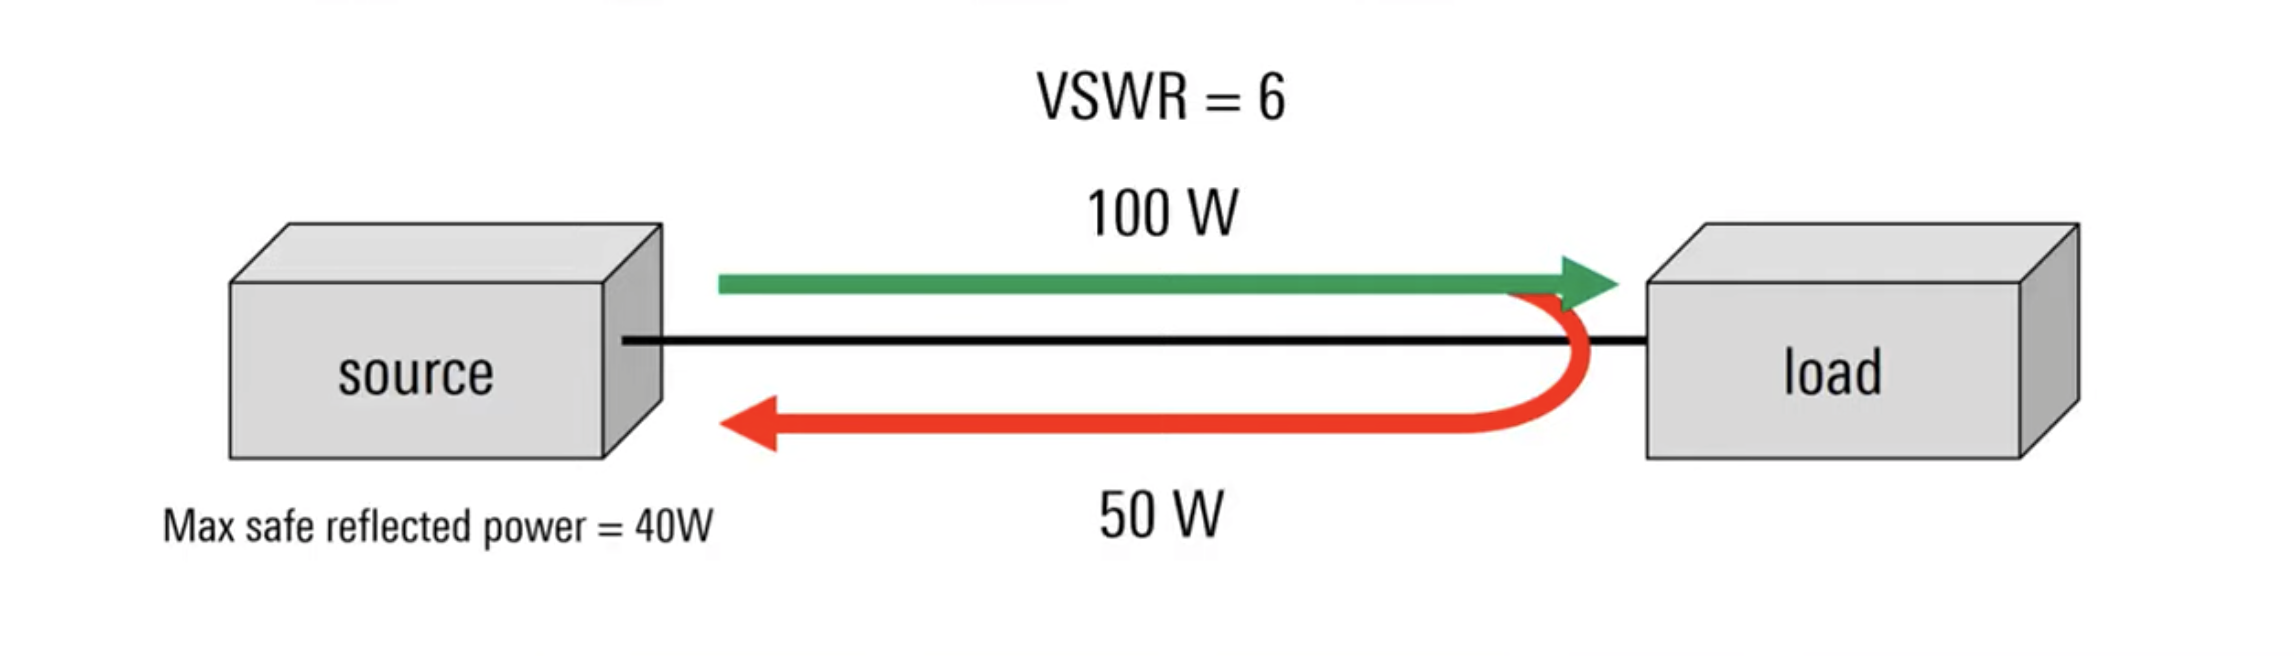
\includegraphics[width=0.75\linewidth]{images/swr.png}
\caption{\label{fig:swr}КСХ антени.}
\end{figure}

Високий КСХ вказує на те, що значна частина потужності сигналу не випромінюється антеною, а відбивається назад у фідер, що може призводити до різних проблем, таких як перегрів передавача, зниження ефективності передачі сигналу і навіть пошкодження обладнання.

\begin{table}[H]
\centering

\begin{tabular}{rcc}
\toprule
\textbf{SWR} & \textbf{\makecell{Voltage \\ reflected (\%)}} & \textbf{\makecell{Power \\ reflected (\%)}} \\
\midrule
1.0:1  & 0   & 0   \\
1.1:1  & 5   & 0.2 \\
1.2:1  & 9   & 0.8 \\
1.3:1  & 13  & 1.7 \\
1.4:1  & 17  & 2.8 \\
1.5:1  & 20  & 4   \\
1.6:1  & 23  & 5.3 \\
1.7:1  & 26  & 6.7 \\
1.8:1  & 29  & 8.2 \\
1.9:1  & 31  & 9.6 \\
\textbf{2.0:1}  & \textbf{33}  & \textbf{11}  \\
2.5:1  & 43  & 18.4 \\
3.0:1  & 50  & 25  \\
4.0:1  & 56  & 36  \\
5.0:1  & 67  & 44.4 \\
10.0:1 & 82  & 67  \\
\bottomrule
\end{tabular}
\caption{Відсоток відбиття напруги і потужності при певних значеннях КСХ.}
\end{table}

\begin{itemize}[noitemsep, topsep=8pt]
\item \textbf{Ідеальне значення КСХ}: Ідеальне значення КСХ --- це 1:1, що означає повне узгодження імпедансів антени і кабеля, при якому всі передані хвилі проходять через антену, і жодна енергія не відбивається назад до передавача.
\item \textbf{Підвищений КСХ}: Якщо КСХ більше 1:1, це означає, що існує певна невідповідність імпедансів, і частина енергії відбивається назад. Наприклад, КСХ 2:1 означає, що 10\% потужності сигналу відбивається, а 90\% передається антеною.
\item \textbf{Значення КСХ}: Зазвичай вважається, що КСХ до 1.5:1 є прийнятним для більшості систем. Вищі значення свідчать про погане узгодження, що може призводити до зменшення ефективності системи і підвищення ризику пошкодження передавача через відбиту потужність.
\end{itemize}


\subsection{Векторий аналіз}

При вимірі характеристик активних і пасивних радіопристроїв (антен, підсилювачів та ін.), а також властивостей різних матеріалів (поглинання та відображення радіохвиль, діелектрична постійна та ін.) широко використовуються векторні аналізатори електричних кіл.

Векторний аналізатор електричних ланцюгів — це прилад, який вимірює характеристики проходження сигналу через пристрій, що тестується, і характеристики відображення сигналу від його портів. Ці характеристики називаються S-параметрами.

Кожен S-параметр містить амплітудно-частотну (АЧХ) і фазо-частотну (ФЧХ) характеристики пристрою, що тестується у відповідному напрямку. Існує багато стандартних способів відображення виміряних S-параметрів на екрані векторного аналізатора електричних кіл. Ви самі можете вибирати, в якому вигляді переглядати результати: у вигляді графіка КСВ або зворотних втрат від частоти, діаграми Сміта, амплітуди, фази, загасання або посилення, групової затримки та ін.


Для того, щоб виконати вимірювання, аналізатор електричних кіл подає на тестований пристрій синусоїдальний сигнал і вимірює сигнал, який відбився, і сигнал, який пройшов через пристрій. Обидва сигнали (відбитий і минулий) відрізнятимуться за амплітудою та фазою від тестового синусоїдального сигналу. Якщо аналізатор електричних кіл може вимірювати лише амплітуду, він \textbf{називається скалярним}. Якщо аналізатор може вимірювати амплітуду і фазу, то він \textbf{називається векторним}. Практично всі сучасні аналізатори електричних кіл є векторними, тому що саме векторний аналізатор дозволяє найбільш повно виміряти характеристики пристрою, що тестується в заданому діапазоні частот.

\begin{figure}[H]
\centering
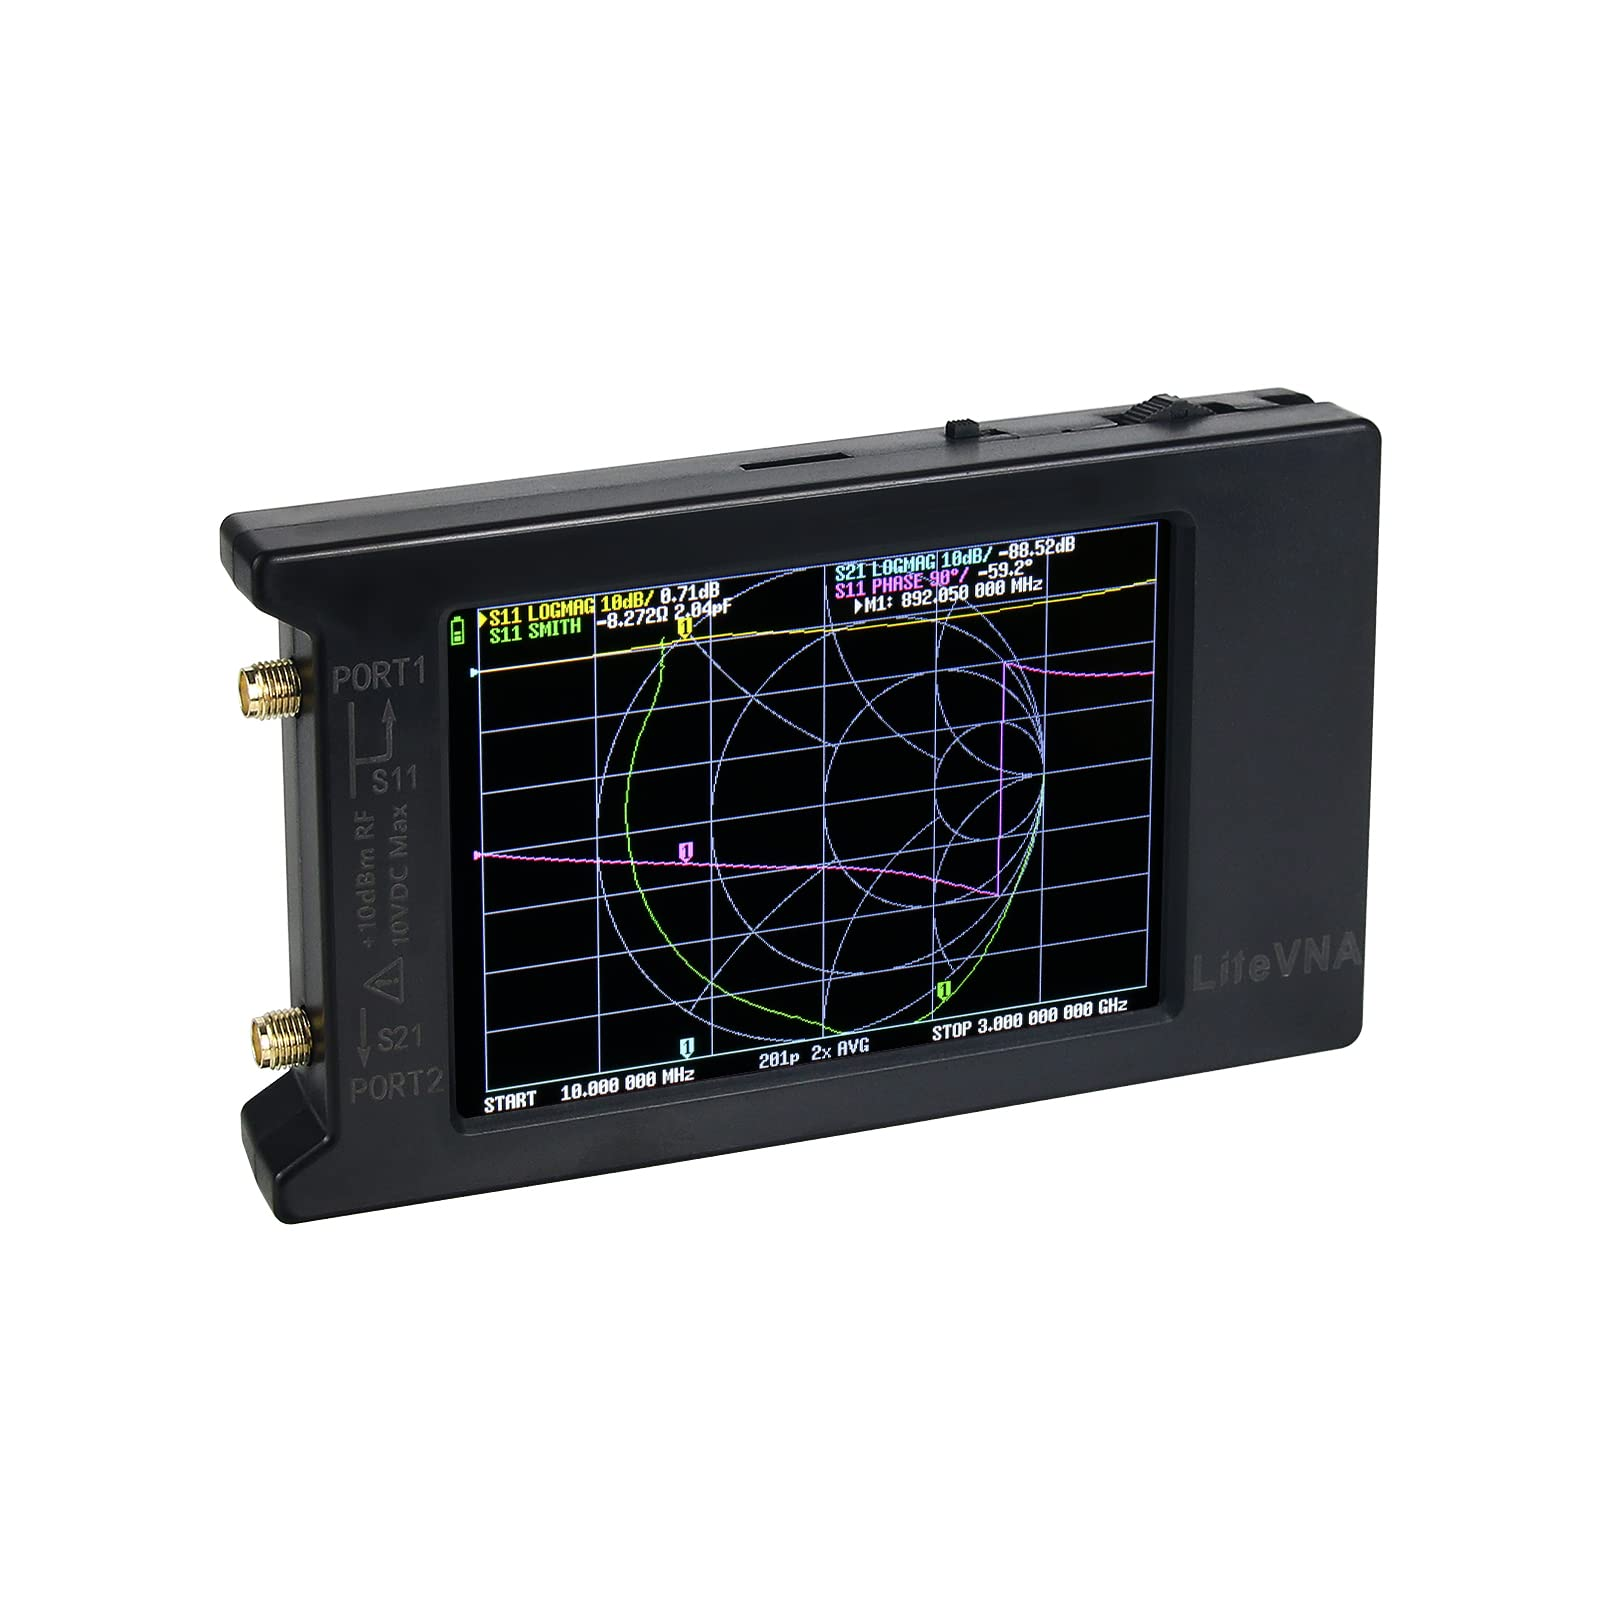
\includegraphics[width=0.6\linewidth]{images/lite-vna.jpg}
\caption{\label{fig:lite-vna}Векторний аналізатор LiteVNA-64.}
\end{figure}

В рамках нашого курсу векторний аналізатор нам цікавий як інструмент, який може вимірювати параметри антен, такі як КСХ (VSWR). Це потрібно для того, щоб якісно оцінити антену і визначити:

\begin{itemize}[noitemsep, topsep=8pt]
\item Чи справна антена.
\item Чи відповідає антена необхідним параметрам.
\end{itemize}

Практичний відеоматеріал стосовно застосування векторного аналізатора та вимірювання різних параметрів, таких як КСХ антени та затухання у кабелі, \href{https://www.youtube.com/watch?v=S4V4TL_5KQg}{доступний за посиланням}.

\subsection{Додаткові матеріали по темі}
\begin{itemize}[noitemsep, topsep=8pt]
\item \href{https://sprotyvg7.com.ua/wp-content/uploads/2023/05/Osnovni-harakterystyky-anten_ukr.pdf}{Основні характеристики і типи польових антен.}
\item \href{https://www.tehencom.com/Categories/Network_Analyzers/Basics/Network_Analyzers_Basics-u.htm}{Що таке векторний аналізатор електричних ланцюгів}.
\item \href{https://www.youtube.com/watch?v=1me_Tz3CFmk}{2 Антенки FPV: діаграма спрямованості і підсилення (gain) в dBi}
\end{itemize}

\section{Пошук джерела сигналу}
 
\textbf{Пеленг} --- це кут між напрямком на північ (географічну або магнітну) і напрямком на об'єкт або джерело сигналу. Пеленг визначається за допомогою спеціальних приладів, які називаються пеленгаторами, і може бути використаний для визначення місцезнаходження джерел радіосигналів або об'єктів у просторі.

Пеленг зазвичай вимірюється в градусах відносно півночі за годинниковою стрілкою, тобто напрямок на північ -- це 0° або 360°, на схід -- 90°, на південь -- 180°, а на захід -- 270°.

В цьому розділі будуть розглянуті основи техніки пошуку напрямку на джерело сигналу та триангуляції.

\subsection{Триангуляція та зведення пеленгів}
\textbf{Триангуляція} --- це метод визначення місцезнаходження об'єкта, що використовується в навігації та радіопеленгуванні. Принцип полягає в тому, що розташування об'єкта обчислюється за допомогою вимірювання кутів до нього з двох або більше відомих точок (точки А та B на мал. \ref{fig:triangulation}). Ці точки формують трикутник, у якому відомі дві точки та кути, що дозволяє обчислити положення третьої точки.

\begin{figure}[H]
\centering
{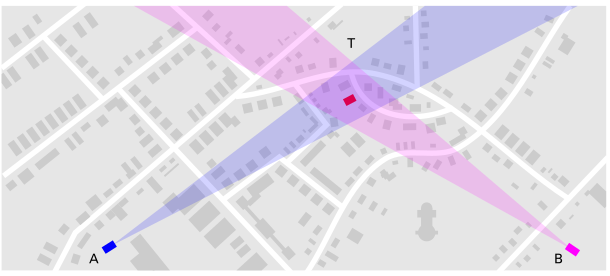
\includegraphics[width=0.6\linewidth]{images/df_triangulation.png}}
\caption{\label{fig:triangulation}Зведення пеленгів.}
\end{figure} 

\textbf{Зведення пеленгів} --- це метод, що використовується для визначення точного місцезнаходження джерела сигналу шляхом вимірювання пеленгів (напрямків) на об'єкт з різних точок спостереження. Кожен пеленг вказує на напрямок, у якому сила сигналу максимальна, і при зведенні кількох пеленгів можна визначити місце, де вони перетинаються, тобто місце розташування передавача. На практиці пеленгування:
\begin{itemize}[noitemsep, topsep=8pt]
\item Кожна пеленгуюча станція вимірює напрямок, з якого надходить сигнал (азимут).
\item Ці пеленги накладаються на карту, де перетин пеленгів з різних точок дає можливість визначити точне місце розташування передавача або об'єкта.	
\end{itemize}


\subsection{Вимірювання напруженості поля}

Одним із найпростіших і найефективніших способів знайти передавач є використання вимірювача напруженості поля з регульованим атенюатором\footnote{В другій частині цього навчального матеріалу у розділі \ref{sec:radio:metter}  наведена схема саморобного вимірювача напруженності поля}. 

\begin{figure}[H]
\centering
{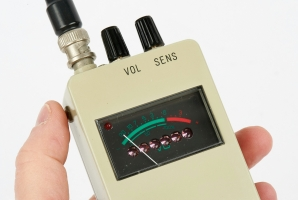
\includegraphics[width=0.6\linewidth]{images/rdf-small.jpg}}
\caption{\label{fig:rds:small}Портативний пристрій для вимірювання напруженності поля.}
\end{figure}

Вимірювання напруженості поля широко використовується й сьогодні, часто в поєднанні з іншими методами радіопеленгації, такими як триангуляція та автоматичне визначення напрямку, особливо на завершальному етапі для виявлення точного місцезнаходження, з якого працює передавач.
 
\subsection{Ручне пеленгування}
Основна форма справжнього пеленгування полягає у використанні (більш-менш) напрямленої антени, такої як диполь, відкрита петля, віконна, Адкока, Ягі або логоперіодична антена. Підключивши антену до приймача і повертаючи її, можна визначити кут максимального або мінімального рівня сигналу.

У випадку портативного приймача та антени перехоплювач може орієнтувати антену в напрямку передавача, поки його не знайде найпотужніший сигнал. Хорошим прикладом сучасної ручної пеленгаційної системи є приймач Rohde \& Schwarz PR-100 у поєднанні з портативною антеною HE-300. 

\begin{figure}[H]
\centering
{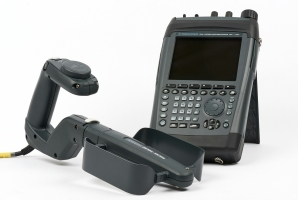
\includegraphics[width=0.6\linewidth]{images/rds-rs-100.jpg}}
\caption{\label{fig:rds:pr100}Портативний пристрій Rohde \& Schwarz PR-100.}
\end{figure}

\subsection{Доплерівське пеленгування}
У системі пеленгування, що базується на ефекті Доплера, антену можна уявити як таку, що обертається з постійною швидкістю в горизонтальній площині, як показано на малюнку нижче. Круговий рух антени \textit{A} викликає частотну модуляцію синусоїдальної форми \textit{fm} у прийнятому сигналі \textit{fc}. Цей ефект відомий як доплерівський зсув частоти. Фаза $\phi$ синусоїдальної модуляції \textit{fm} буде визначатися кутом падіння $\alpha$ прийнятого сигналу \textit{fc}. Порівнюючи фазу джерела керування двигуном та демодульованого сигналу, можна визначити початковий кут падіння прийнятого сигналу.

\begin{figure}[H]
\centering
{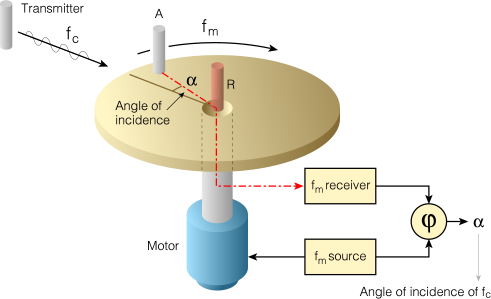
\includegraphics[width=0.6\linewidth]{images/rdf-dopler.png}}
\caption{\label{fig:rdf:dopler}Cхематичне зображення принципу вимірювання напрямку джерела випромінювання використовуючи ефект Доплера.}
\end{figure}

На практиці обертання антени імітується електронним комутуванням (перемиканням) між кількома дискретними антенами, рівномірно розташованими по колу. Зазвичай, більшість систем складається з чотирьох або восьми дискретних антен. Крім того, референсна антена \textit{R} часто розташовується в центрі кола для прийому у звичайному режимі. У цьому випадку референсний сигнал використовується для усунення частотної модуляції, викликаної голосом, щоб фаза частотної модуляції, викликаної ефектом Доплера \textit{fm}, могла бути визначена більш точно.

\subsection{Принцип Homer}

Принцип Homer\footnote{Також можна зустріти цей метод під назвою \textit{Монопульс на основі порівняння амплітуд}.} складається з двох спрямованих антен, які направлені трохи вбік від центру. Використовуючи діаграми спрямованості антен і швидко перемикаючись між ними, можна виміряти стрибки сили сигналу, за винятком випадку, коли передавач знаходиться прямо попереду, в такому разі сила сигналу на обох антенах буде однаковою (точка P мал. \ref{fig:homer}).

\begin{figure}[H]
\centering
{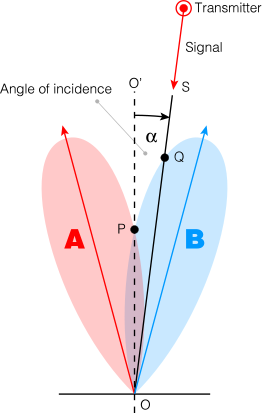
\includegraphics[width=0.3\linewidth]{images/homer.png}}
\caption{\label{fig:homer}Cхематичне розташування антен.}
\end{figure}

Діаграма вище показує, як це працює. Дві антени \texttt{A} і \texttt{B} мають однакові діаграми спрямованості, але вони спрямовані трохи в різні боки, наприклад, на \texttt{$+15^\circ$°} і \texttt{$-15^\circ$} у напрямку джерела випромінювання. Коли передавач знаходиться прямо попереду, сигнал від обох антен буде однаковим \texttt{A=B}, і різниці у силі сигналу не буде. Це показано в точці P на діаграмі вище.

\begin{figure}[H]
\centering
{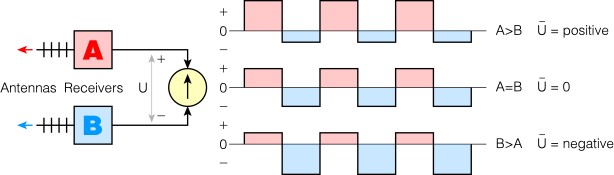
\includegraphics[width=0.7\linewidth]{images/homer_meter.png}}
\caption{\label{fig:homer:meter}Функціональна схема методу Гомера.}
\end{figure}

Коли сила сигналу між двома антенами різна (наприклад, коли \texttt{B>A}), то рівні сигналів від антен будуть також різними і ця різниця є мірою для визначення кута надходження сигналу. Точка \texttt{Q} у прикладі. Діаграма вище показує, як сила сигналу з обох антен впливає на вихідні показники. У стані спокою \texttt{A=B} стрілка індикатора вказує вгору \texttt{0V}.

\begin{figure}[H]
\centering
{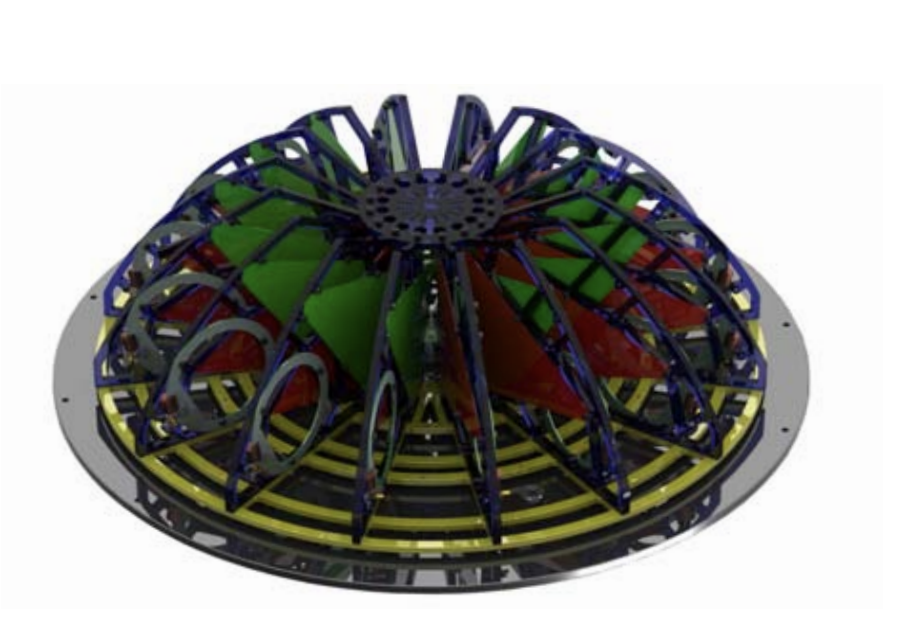
\includegraphics[width=0.6\linewidth]{images/isolog-3d-160.png}}
\caption{\label{fig:isolog-3d}Масив антен встановлених на єдиному шасі. Антена IsoLOG 3D 160 від \href{https://aaronia.com/en/produkte/antennas/isolog-3d-df}{Aaronia}.}
\end{figure}

На базі цього рішення можна побудувати антену яка здатна визначати не тільки напрямок об'єкту по горизонталі(азимут відносно півночі), а також кут по вертикалі. На мал. \ref{fig:isolog-3d} зображено масив із антен поєднаних у єдину систему. Комплекс із застосуванням таких антен може обчислювати місцезнаходження (по зведеному пелелегу) і висоту джерела сигналу. 

\subsection{Кореляційний інтерферометр}
Кореляційний інтерферометр використовує дві або (переважно) три ідентичні антени та приймачі, розташовані на відомих відстанях, а також сигнал від (четвертої) референсної антени. Ці сигнали аналізуються за допомогою комп'ютерної системи, використовуючи передові математичні методи, такі як швидке перетворення Фур'є (FFT). Фаза сигналів використовується для розрахунку азимута на передавач.

\begin{figure}[H]
\centering
{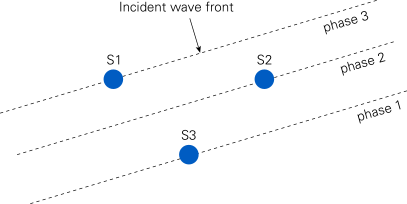
\includegraphics[width=0.5\linewidth]{images/df_int_wave.png}}
\caption{Cхематичне зображення послідовності надходження сигнала на антени інтерферометра.}
\end{figure}

Ілюстрація вище показує, як це працює для системи з трьома антенами, розташованими у формі трикутника. Антени підключені до трьох ідентичних приймачів, які налаштовані паралельно за допомогою спільного локального осцилятора, що контролюється комп'ютерною системою. Сигнали з трьох приймачів перетворюються в цифровий формат (тобто оцифровуються), а потім передаються до комп'ютера.

\begin{figure}[H]
\centering
{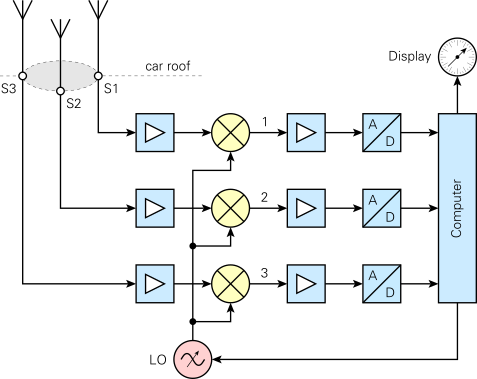
\includegraphics[width=0.6\linewidth]{images/df_int.png}}
\caption{Функціональна схема інтерферометра.}
\end{figure}
 
% https://www.cryptomuseum.com/df/df.htm

\subsection{Додаткові матеріали по темі}
\begin{itemize}[noitemsep, topsep=8pt]
\item \href{https://www.youtube.com/watch?v=N8rZIAHxAH4}{An Introduction to Direction Finding}
\item \href{https://www.cryptomuseum.com/df/df.htm}{Radio Direction Finding}	
\item \href{http://www.homingin.com/newdopant.html}{Wide-Range Antenna Arrays For the Roanoke Doppler}
\end{itemize}


\begin{thebibliography}{99}

\bibitem{bib:rothammel}
К. Ротгамель, \textit{Антени}, 2005.

\bibitem{bib:pistolikors}
А. Пистолькорс. \textit{Антени}, 1947.

\bibitem{bib:kocherzhevskij}
Г. Кочержевський, \textit{Антено-фидерні пристрої}, 1981

\end{thebibliography}

\end{document}